
\setsecnumdepth{subsection}

\begin{alttitles}

\chapter{Eigenapplications}

We end this book with a few more ultra-cool real-world applications of linear
algebra. Unlike those in Chapter~\ref{ch:apps}, though, these will all involve
the \textbf{eigenvalue} concepts you learned in Chapter~\ref{ch:eigen}. Our
new ability to penetrate to the heart of a matrix and understand its inner
structure will enable us to do things we could only dream about before.

\pagebreak

\renewcommand{\thesubsection}{V\arabic{subsection}.}%... from subsections
\section{Video compression}

Imagine you owned a business, and you needed to send a $7\times 7$ matrix over
the Internet to one of your customers. Say, this matrix:

\vspace{-.15in}
\begin{align*}
M_1 = 
\begingroup
\renewcommand*{\arraystretch}{1.2}
\begin{bmatrix}
5 & -1 & 45 & 16 & 16 & 3 & 37 \\
3 & -9 & 9  & 27 & -100 & 24 & 601 \\
13 & 0 & 2  & 13 & -18 & 21 & 11 \\
-4 & 33 & 9  & 1 & 4 & 14 & 50 \\
-21 & 51 & 9  & 17 & 5 & 73 & -5 \\
31 & -5 & 9  & -99 & -22 & 1 & 7 \\
6 & 8 & 9  & 24 & 8 & 8 & 8 \\
\end{bmatrix}.
\endgroup
\end{align*}
\vspace{-.15in}

How many numbers in total would you have to send your customer to communicate
the information in this matrix?

Easy question. There are 49 entries in a 7-by-7 matrix, so you need to send 49
numbers. Duh.

\medskip

Now suppose you wanted to send this matrix instead:

\vspace{-.15in}
\begin{align*}
M_2 = 
\begingroup
\renewcommand*{\arraystretch}{1.2}
\begin{bmatrix}
5 & 5 & 10 & -5 & 20 & 500 & 2\frac{1}{2} \\
3 & 3 & 6 & -3 & 12 & 300 & 1\frac{1}{2} \\
13 & 13 & 26 & -13 & 52 & 1300 & 6\frac{1}{2} \\
-4 & -4 & -8 & 4 & -16 & -400 & -2 \\
-21 & -21 & -42 & 21 & -84 & -2100 & -10\frac{1}{2} \\
31 & 31 & 62 & -31 & 124 & 3100 & 15\frac{1}{2} \\
6 & 6 & 12 & -6 & 24 & 600 & 3 \\
\end{bmatrix}.
\endgroup
\end{align*}
\vspace{-.15in}

How many numbers would you have to send this time?

If you answered, ``again, 49,'' take another look. $M_2$ is way different than
$M_1$, because it has a very regular structure. Look at $M_2$'s first
(leftmost) column. Then realize that its second column is identical to the
first. Then further realize that its third column is exactly \textit{twice} the
first. And its fourth column is \textit{negative} the first. And its last three
columns are four times, a hundred times, and one-half times the first column,
respectively.

So if your customer knew the matrix would have this type of structure, I claim
you could send them all the necessary information in just \textit{fourteen}
numbers instead of 42. Here's how:

\begin{compactenum}
\item First, send them the first column: $[\ 5\ \ 3\ \ 13\ \ -4\ \ -21\ \ 31\ \
6\ ]$. That's seven numbers.
\index{Oakenshield, Thorin}
\item Then, send them the multiplier for each of the other columns. Namely, $[\
1\ \ 1\ \ 2\ \ -1\ \ 4\ \ 100\ \ \frac{1}{2}\ ]$. That, too, is seven
numbers.\footnote{Yeah, yeah, I know we could omit the first ``1'' in this
second set of seven, because the customer will know that the first column
should be multiplied by 1 without us having to tell them. That's a detail, and
it's actually messier to take advantage of that. Thirteen is unlucky anyway --
ask Thorin Oakenshield if you don't believe me.}

\end{compactenum}

\index{outer product}

From these fourteen numbers alone, the customer can reconstruct the original
matrix. All they have to do is compute the outer product (recall
p.~\pageref{outerProduct}) of the two 7-element vectors they received:

\vspace{-.15in}
\begin{gather*}
\begin{bmatrix}
5 \\ 3 \\ 13 \\ -4 \\ -21 \\ 31 \\ 6 \\
\end{bmatrix} \ \textrm{\textbullet} \ 
\begin{bmatrix}
1 & 1 & 2 & -1 & 4 & 100 & \frac{1}{2} \\
\end{bmatrix} =\\
\begingroup
\renewcommand*{\arraystretch}{1.2}
\begin{bmatrix}
5 & 5 & 10 & -5 & 20 & 500 & 2\frac{1}{2} \\
3 & 3 & 6 & -3 & 12 & 300 & 1\frac{1}{2} \\
13 & 13 & 26 & -13 & 52 & 1300 & 6\frac{1}{2} \\
-4 & -4 & -8 & 4 & -16 & -400 & -2 \\
-21 & -21 & -42 & 21 & -84 & -2100 & -10\frac{1}{2} \\
31 & 31 & 62 & -31 & 124 & 3100 & 15\frac{1}{2} \\
6 & 6 & 12 & -6 & 24 & 600 & 3 \\
\end{bmatrix}.
\endgroup
\end{gather*}
\vspace{-.15in}

\medskip
\label{rank-deficient}

What's going on here? Simply put, $M_2$ has \textit{less information} in it
than $M_1$ does, despite the fact that they are ostensibly the same size. In
fact, you may have realized that $M_2$ is a \textbf{rank-1} matrix. It has only
one linearly independent column: all the others are simply (scaled) copies of
it. This is what a rank-deficient matrix fundamentally is: a matrix that can
have some of its entries ``squeezed'' out of it without losing any information.

\smallskip

$M_1$ and $M_2$ represent the far extremes of this phenomenon. $M_1$ is full
rank (rank-7), and $M_2$ is just rank-1. In general, a $7\times 7$
rank-deficient matrix might not be \textit{as} deficient as $M_2$ is: it could
have a rank anywhere from 1 to 6.

\smallskip

Incidentally, 14 numbers might not seem like that big a savings over 49 (it's
only 3.5 times fewer entries), but consider what happens as the matrix gets
larger. Suppose it were $1920\times 1920$. Transmitting a rank-1 matrix of that
size would require $1920+1920=$\ 3,840 numbers to go across the wire. But a
full-rank matrix of that size would need \textit{3,686,400} entries. That's
nearly 1,000 times as much data.

\subsection{Enter Netflix}

\index{frame (of a video)}
\index{gray scale}
\index{bit / byte}

Now what's the application here? Well, it's probably one you use every day.
Suppose your aforementioned business is a video streaming service, and your
customer is watching one of your videos. The matrix we've been talking about is
one \textbf{frame} of this video. For simplicity, we'll consider images
(frames) that are in \textbf{gray scale} rather than color. Each \textbf{pixel}
of the image is represented by a single number on some scale: perhaps 0
indicates a pitch black pixel in the current frame, and 255 is bright white,
and all the numbers in between are shades of gray.\footnote{Why a range of 0
through 255? Because as you may remember from Chapters 6 and 7 of \textit{A
Cool Brisk Walk}, that's how many different values can fit in a single byte (8
bits) of data.}

If each frame of our movie is a $1920\times 1920$-pixel square\footnote{At this
point it may occur to you that when you watch a movie, your screen typically
isn't perfectly square, but rectangular. Its \index{aspect ratio}
\textbf{aspect ratio} (width-to-height) might be, say, 1.875:1, which yields a
$1920\times 1024$ canvas. \\ \indent When your matrix isn't square, instead of using
the eigenvalue decomposition, as we learned last chapter, we can use the
\index{singular value decomposition (SVD)} \textbf{singular value decomposition
(SVD)}, a very closely related technique. In fact, the ``singular values'' and
``singular vectors'' that the SVD gives you are exactly the same thing as
eigenvalues and eigenvectors for a non-square matrix.}, and we're shoveling 30
frames per second at our viewer, that would be about 105 Megabytes of
information \textit{every second} we'd be trying to send. The Internet
ain't got no time for that.

So we'd like to instead send a compressed version of each frame: a matrix whose
rank is far less than 1,920 and yet which looks pretty close to the original.
Our problem thus reduces to: \textit{what matrix, of the same size as the
original image's matrix but of at most rank-k (for some number k) is the
``closest'' to the original?}

\subsection{Yet another norm}

\index{Frobenius norm}
\index{norm (of a matrix)}
\index{Euclidean norm}

First, we have to settle on what we mean by one matrix being ``close'' to
another. Here, we'll subtract one matrix from the other, and then take the
\textbf{Frobenius norm} of this difference. Subtracting matrices, of course, is
just the inverse of adding them (p.~\pageref{matrixAddition}): we do it element
by element and get a matrix of the differences. The ``Frobenius norm'' (which
always sounded to me like a character from a Willy Wonka story, btw) is just
what you would expect it to be: the square-root of the sum of all these squared
differences. In fact it's exactly like the Euclidean norm of a vector
(p.~\pageref{Euclideannorm}), except that we have a two-dimensional pane of
entries to work with instead of just a one-dimensional list.

To be concrete, let's say we have a matrix $M$, and an ``approximation'' to
matrix $M$ called $\hat{M}$, with the following values:

\vspace{-.15in}
\begin{align*}
M =
\begin{bmatrix}
17 & 2 \\
-3 & 6 \\
\end{bmatrix}, \quad
\hat{M} =
\begin{bmatrix}
14 & 4 \\
-5 & -1 \\
\end{bmatrix}, 
\end{align*}
\vspace{-.15in}

How ``close'' are these two matrices to each other? To quantify this, we first
subtract one from the other (doesn't matter which order):

\vspace{-.15in}
\begin{align*}
M - \hat{M} =
\begin{bmatrix}
3 & -2 \\
2 & 7 \\
\end{bmatrix}.
\end{align*}
\vspace{-.15in}

And then we take the square-root of the sum of the squared entries to give us
the Frobenius norm:

\vspace{-.15in}
\begin{align*}
{\left\lVert{M - \hat{M}}\right\rVert_F} =
\sqrt{3^2 + -2^2 + 2^2 + 7^2} = 8.124.
\end{align*}
\vspace{-.15in}

This measure passes a quick sanity check: the further apart the entries of $M$
and $\hat{M}$ at a particular row and column, the larger the difference that is
added towards the Frobenius norm. So this metric gives pairs of matrices whose
entries are more similar to each other a lower overall norm, indicating a
higher similarity.

\subsection{Best low-rank matrix approximations}

\index{dominant eigenvector}

And now for our eigenstuff. Recall (p.~\pageref{theScoopAboutEigenvectors} and
following) that every eigenvector of a matrix has a corresponding eigenvalue,
and that we could arrange these eigenvectors by decreasing eigenvalue if we
like. The one with the largest eigenvalue had the special name ``dominant
eigenvector.'' I'll also refer to ``the top eigenvector,'' ``the top two
eigenvectors,'' ``the top ten eigenvectors,'' and so forth, by which I just
mean ``the $k$ eigenvectors with the highest eigenvalues.''

Okay. It turns out that the best rank-1 approximation to a square matrix (where
``best'' means ``closest to the original when using the Frobenius norm'') is
\textit{the dominant eigenvector, times its eigenvalue, times the transpose of
the dominant eigenvector.} To illustrate, let's say we had this $5\times 5$
matrix\footnote{You may notice that this example matrix happens to be
\textit{symmetric}. Things actually get slightly weird for non-symmetric
matrices, in which case you can again turn to the SVD,\index{singular value
decomposition (SVD)} which is almost the same thing as the
\index{eigendecomposition (of a matrix)} eigendecomposition.}:

\vspace{-.15in}
\label{Amatrix}
\begin{align*}
A =
\begin{bmatrix}
12 & 2 & 1 & 9 & 13 \\
2 & 20 & 12 & 7 & 5 \\
1 & 12 & 6 & -4 & 5 \\
9 & 7 & -4 & 8 & 8 \\
13 & 5 & 5 & 8 & 13 \\
\end{bmatrix}
,
\end{align*}
\vspace{-.15in}

and we wanted the best rank-1 approximation to it. We ask Python for its
dominant eigenvector, and the corresponding eigenvalue, and get this:

\vspace{-.15in}
\begin{align*}
\overrightarrow{x_1} = 
\begin{bmatrix}
.462 \\ .538 \\ .257 \\ .38 \\ .535 \\
\end{bmatrix}, \quad
\lambda_1 = 37.363.
\end{align*}
\vspace{-.15in}

Multiplying these out as indicated above, we get:

\vspace{-.15in}
\begin{gather*}
\overrightarrow{x_1} \ \textrm{\textbullet} \  \begin{bmatrix} \lambda_1
\end{bmatrix} \ \textrm{\textbullet} \  \overrightarrow{x_1}^\intercal =\\
\begin{bmatrix}
.462 \\ .538 \\ .257 \\ .38 \\ .535 \\
\end{bmatrix} \ \textrm{\textbullet}\ 
\begin{bmatrix}
37.363
\end{bmatrix} \ \textrm{\textbullet}\ 
\begin{bmatrix}
.462 & .538 & .257 & .38 & .535 \\
\end{bmatrix} = \\
\begin{bmatrix}
7.963 & 9.288 & 4.441 & 6.563 & 9.222\\
9.288 & 10.834 & 5.18 & 7.655 & 10.757\\
4.441 & 5.18 & 2.477 & 3.66 & 5.143\\
6.563 & 7.655 & 3.66 & 5.409 & 7.6 \\
9.222 & 10.757 & 5.143 & 7.6 & 10.68 \\
\end{bmatrix}.
\end{gather*}
\vspace{-.05in}

\index{Spectral Theorem}

Take careful note to see that \textit{this is actually the \textbf{Spectral
Theorem} in action} (from p.~\pageref{SpectralTheorem}) but using only a subset
of the eigenvectors/eigenvalues (namely, the top one) instead of all of them.
(This is why I put the top eigenvalue, 37.363, into a $1\times 1$ matrix in the
equation above -- to help you see that connection.)

\medskip

Now how close is this approximation to our original $A$ matrix? Not that great,
actually. If you run your eyes over the entries, and compare to $A$
(p.~\pageref{Amatrix}) it doesn't even look like it's trying very hard. The
Frobenius norm of the difference between the two, by the way, is a whopping
573.04, which tells you that limiting ourselves to rank-1 isn't producing a
very good approximation. We wouldn't want to send such an image to our viewer,
even though it would only take 10 bytes instead of 25, because they might not
even know whether they were on HBO or the Disney Channel.

\bigskip

Okay, let's move up to rank-2 then. What's the closest rank-2 matrix to our
original? Python says the second highest eigenvalue (and its eigenvector) are:

\vspace{-.15in}
\begin{align*}
\overrightarrow{x_2} = 
\begin{bmatrix}
-.458 \\ .658 \\ .448 \\ -.266 \\ -.293 \\
\end{bmatrix}, \quad
\lambda_2 = 27.712.
\end{align*}
\vspace{-.15in}

Adding this second eigenvector into the mix, we get:

\vspace{-.15in}
\begin{gather*}
\begin{bmatrix}
| & | \\[6pt]
\overrightarrow{\textbf{x}_{1}} &
\overrightarrow{\textbf{x}_{2}} \\
| & | \\[6pt]
\end{bmatrix} \ \textrm{\textbullet}\ 
\begin{bmatrix}
\lambda_1 & 0 \\
0 & \lambda_2 \\
\end{bmatrix} \ \textrm{\textbullet}\ 
\begin{bmatrix}
| & | \\[6pt]
\overrightarrow{\textbf{x}_{1}} &
\overrightarrow{\textbf{x}_{2}} \\
| & | \\[6pt]
\end{bmatrix}^\intercal = \\
\small
\begingroup
\setlength\arraycolsep{2pt}
\begin{bmatrix}
.462 & -.458 \\
.538 & .658 \\
.257 & .448 \\
.38 & -.266 \\
.535 & -.293 \\
\end{bmatrix} \ \textrm{\textbullet}\ 
\begin{bmatrix}
37.363 & 0 \\
0 & 27.712 \\
\end{bmatrix} \ \textrm{\textbullet}\ 
\begin{bmatrix}
.462 & .538 & .257 & .38 & .535 \\
-.458 & .658 & .448 & -.266 & -.293 \\
\end{bmatrix}\endgroup\\
=
\begin{bmatrix}
 12.515 & 2.748 & -0.011 & 9.211 & 12.138 \\
 2.748 & 20.231 & 11.577 & 3.849 & 6.567 \\
 -0.011 & 11.577 & 6.831 & 1.07 & 2.291 \\
 9.211 & 3.849 & 1.07 & 6.95 & 9.297 \\
 12.138 & 6.567 & 2.291 & 9.297 & 12.548 \\
\end{bmatrix}.
\end{gather*}
\vspace{-.05in}

Now we're talking. Flip back and forth between those numbers and the original
$A$ on p.~\pageref{Amatrix}, and you'll see that with just two eigenvectors,
we're starting to get a remarkably close approximation. Frobenius just
plummeted to 101.62. Repeating this for the best rank-3 approximation, we get:

\vspace{-.15in}
\begin{gather*}
\begin{bmatrix}
| & | & | \\[6pt]
\overrightarrow{\textbf{x}_{1}} &
\overrightarrow{\textbf{x}_{2}} &
\overrightarrow{\textbf{x}_{3}} \\
| & | & | \\[6pt]
\end{bmatrix} \ \textrm{\textbullet}\ 
\begin{bmatrix}
\lambda_1 & 0 & 0 \\
0 & \lambda_2 & 0 \\
0 & 0 & \lambda_3 \\
\end{bmatrix} \ \textrm{\textbullet}\ 
\begin{bmatrix}
| & | & | \\[6pt]
\overrightarrow{\textbf{x}_{1}} &
\overrightarrow{\textbf{x}_{2}} &
\overrightarrow{\textbf{x}_{3}} \\
| & | & | \\[6pt]
\end{bmatrix}^\intercal = \\
\begingroup
\setlength\arraycolsep{2pt}
\footnotesize
\begin{bmatrix}
.462 & -.458 & .156 \\
.538 & .658 & -.33 \\
.257 & .448 & .525 \\
.38 & -.266 & -.651 \\
.535 & -.293 & .408 \\
\end{bmatrix} \ \textrm{\textbullet}\ 
\begin{bmatrix}
37.363 & 0 & 0 \\
0 & 27.712 & 0 \\
0 & 0 & 7.6 \\
\end{bmatrix} \ \textrm{\textbullet}\ 
\begin{bmatrix}
.462 & .538 & .257 & .38 & .535 \\
-.458 & .658 & .448 & -.266 & -.293 \\
.156 & -.33 & .525 & -.651 & .408 \\
\end{bmatrix} \endgroup \\
=
\begin{bmatrix}
12.701 & 2.356 & 0.612 & 8.438 & 12.623 \\
 2.356 & 21.06 & 10.259 & 5.484 & 5.542 \\
 0.612 & 10.259 & 8.925 & -1.528 & 3.921 \\
 8.438 & 5.484 & -1.528 & 10.173 & 7.276 \\
 12.623 & 5.542 & 3.921 & 7.276 & 13.815 \\
\end{bmatrix},
\end{gather*}
\vspace{-.15in}

which is even closer, with a Frobenius norm of just 59.07.

\bigskip

Each time we add another eigenvector, we give our approximation another degree
of freedom which it can use to bend closer to the original. And finally, if we
use all 5, we of course get the original matrix back:

\vspace{-.15in}
\footnotesize
\begin{gather*}
\begin{bmatrix}
| & | & | & | & | \\[6pt]
\overrightarrow{\textbf{x}_{1}} &
\overrightarrow{\textbf{x}_{2}} &
\overrightarrow{\textbf{x}_{3}} &
\overrightarrow{\textbf{x}_{4}} &
\overrightarrow{\textbf{x}_{3}} \\
| & | & | & | & | \\[6pt]
\end{bmatrix} \ \textrm{\textbullet}\ 
\begin{bmatrix}
\lambda_1 & 0 & 0 & 0 & 0 \\
0 & \lambda_2 & 0 & 0 & 0 \\
0 & 0 & \lambda_3 & 0 & 0 \\
0 & 0 & 0 & \lambda_4 & 0 \\
0 & 0 & 0 & 0 & \lambda_5 \\
\end{bmatrix} \ \textrm{\textbullet}\ 
\begin{bmatrix}
| & | & | & | & | \\[6pt]
\overrightarrow{\textbf{x}_{1}} &
\overrightarrow{\textbf{x}_{2}} &
\overrightarrow{\textbf{x}_{3}} &
\overrightarrow{\textbf{x}_{4}} &
\overrightarrow{\textbf{x}_{5}} \\
| & | & | & | & | \\[6pt]
\end{bmatrix}^\intercal = \\
\begingroup
\setlength\arraycolsep{2pt}
\footnotesize
\begin{bmatrix}
-0.462 & -0.458 & 0.156 & 0.735 & -0.109 \\
 -0.538 & 0.658 & -0.33 & 0.082 & -0.402 \\
 -0.257 & 0.448 & 0.525 & 0.105 & 0.668 \\
 -0.38 & -0.266 & -0.651 & -0.181 & 0.572 \\
 -0.535 & -0.293 & 0.408 & -0.639 & -0.23 &  \\
\end{bmatrix}\endgroup \ \textrm{\textbullet} \quad \quad \quad \quad \quad \quad \quad \quad
\quad \quad
\\
\quad \quad \quad \quad \quad \quad \quad \quad
\quad \quad
\begingroup
\setlength\arraycolsep{2pt}
\begin{bmatrix}
37.363 & 0 & 0 & 0 & 0 \\
0 & 27.712 & 0 & 0 & 0 \\
0 & 0 & 7.599 & 0 & 0 \\
0 & 0 & 0 & -.151 & 0 \\
0 & 0 & 0 & 0 &  -6.523 \\
\end{bmatrix}\endgroup \ \textrm{\textbullet} \quad \quad \quad \quad \quad \quad \quad \quad
\quad \quad
\\
\end{gather*}
\pagebreak
\begin{gather*}
\quad \quad \quad \quad \quad \quad \quad \quad \quad \quad \quad \quad
\begingroup
\setlength\arraycolsep{2pt}
\begin{bmatrix}
-0.462 & -0.538 & -0.257 & -0.38 & -0.535 \\
 -0.458 & 0.658 & 0.448 & -0.266 & -0.293 \\
 0.156 & -0.33 & 0.525 & -0.651 & 0.408 \\
 0.735 & 0.082 & 0.105 & -0.181 & -0.639 \\
 -0.109 & -0.402 & 0.668 & 0.572 & -0.23 \\
\end{bmatrix}\endgroup = \\
\normalsize
\begin{bmatrix}
12 & 2 & 1 & 9 & 13 \\
2 & 20 & 12 & 7 & 5 \\
1 & 12 & 6 & -4 & 5 \\
9 & 7 & -4 & 8 & 8 \\
13 & 5 & 5 & 8 & 13 \\
\end{bmatrix} = A \quad \checkmark
\end{gather*}
\vspace{-.05in}

\normalsize
by the Spectral Theorem. (And a Frobenius norm of 0.)

\bigskip
\bigskip

Finally, let's look at this work on an actual image.
Figure~\ref{fig:stormtrooper} shows a $1800\times 1800$ gray scale still
frame from a movie. At 1 byte (8 bits) per pixel, the entire original image
would take 3.24 MBytes to transmit in full. That's a lot of data for one frame
of a movie that the viewer will only see for $\frac{1}{30}^\textrm{th}$ of a
second.

\begin{figure}[hb]
\centering
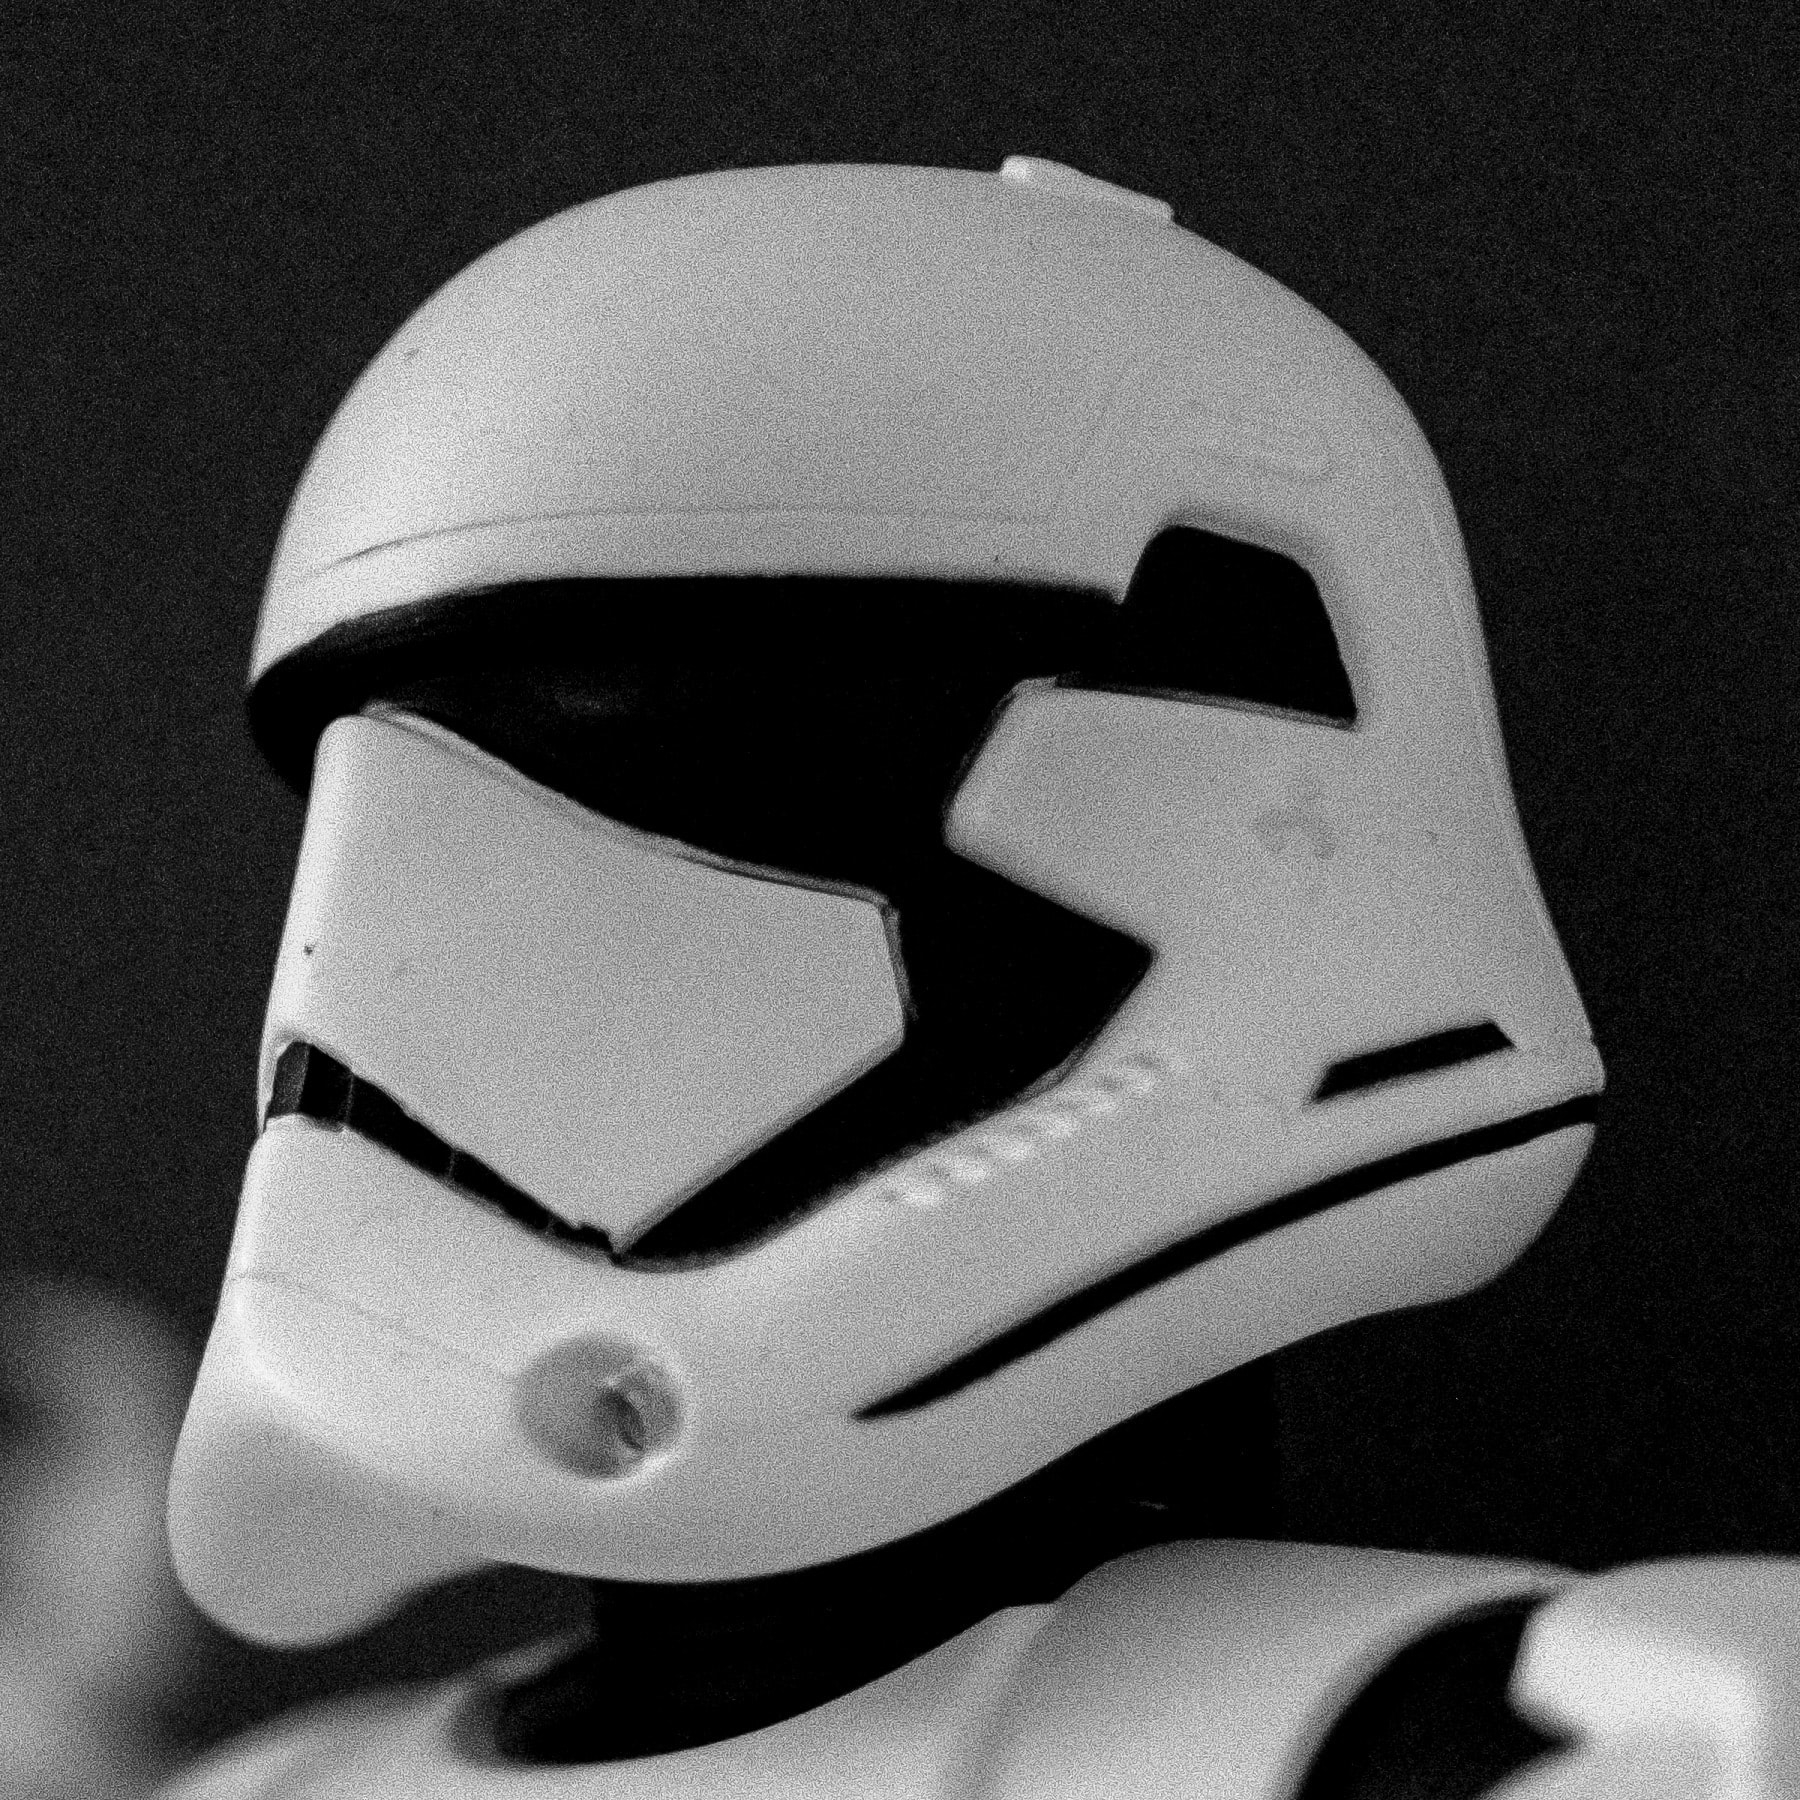
\includegraphics[width=0.5\textwidth]{stormtrooper.png}
\caption{A 3,240,000-byte gray scale image.}
\label{fig:stormtrooper}
\end{figure}

Let's see if we can do better. Figure~\ref{fig:approximations} starts with a
lowly rank-1 matrix (using just the dominant eigenvector), and then increases
the rank as the images move left-to-right down the page.

\begin{figure}[H]
\centering
\begin{tabular}{ccc}
\scriptsize{Rank-1 (3600 bytes)} &
\scriptsize{Rank-2 (7200 bytes)} &
\scriptsize{Rank-3 (10,800 bytes)} \\

\includegraphics[width=0.3\textwidth]{approx01.png} &

\includegraphics[width=0.3\textwidth]{approx02.png} &

\includegraphics[width=0.3\textwidth]{approx03.png}\\
\smallskip
\scriptsize{Rank-6 (21,600 bytes)} &
\scriptsize{Rank-9 (32,400 bytes)} &
\scriptsize{Rank-12 (43,200 bytes)} \\
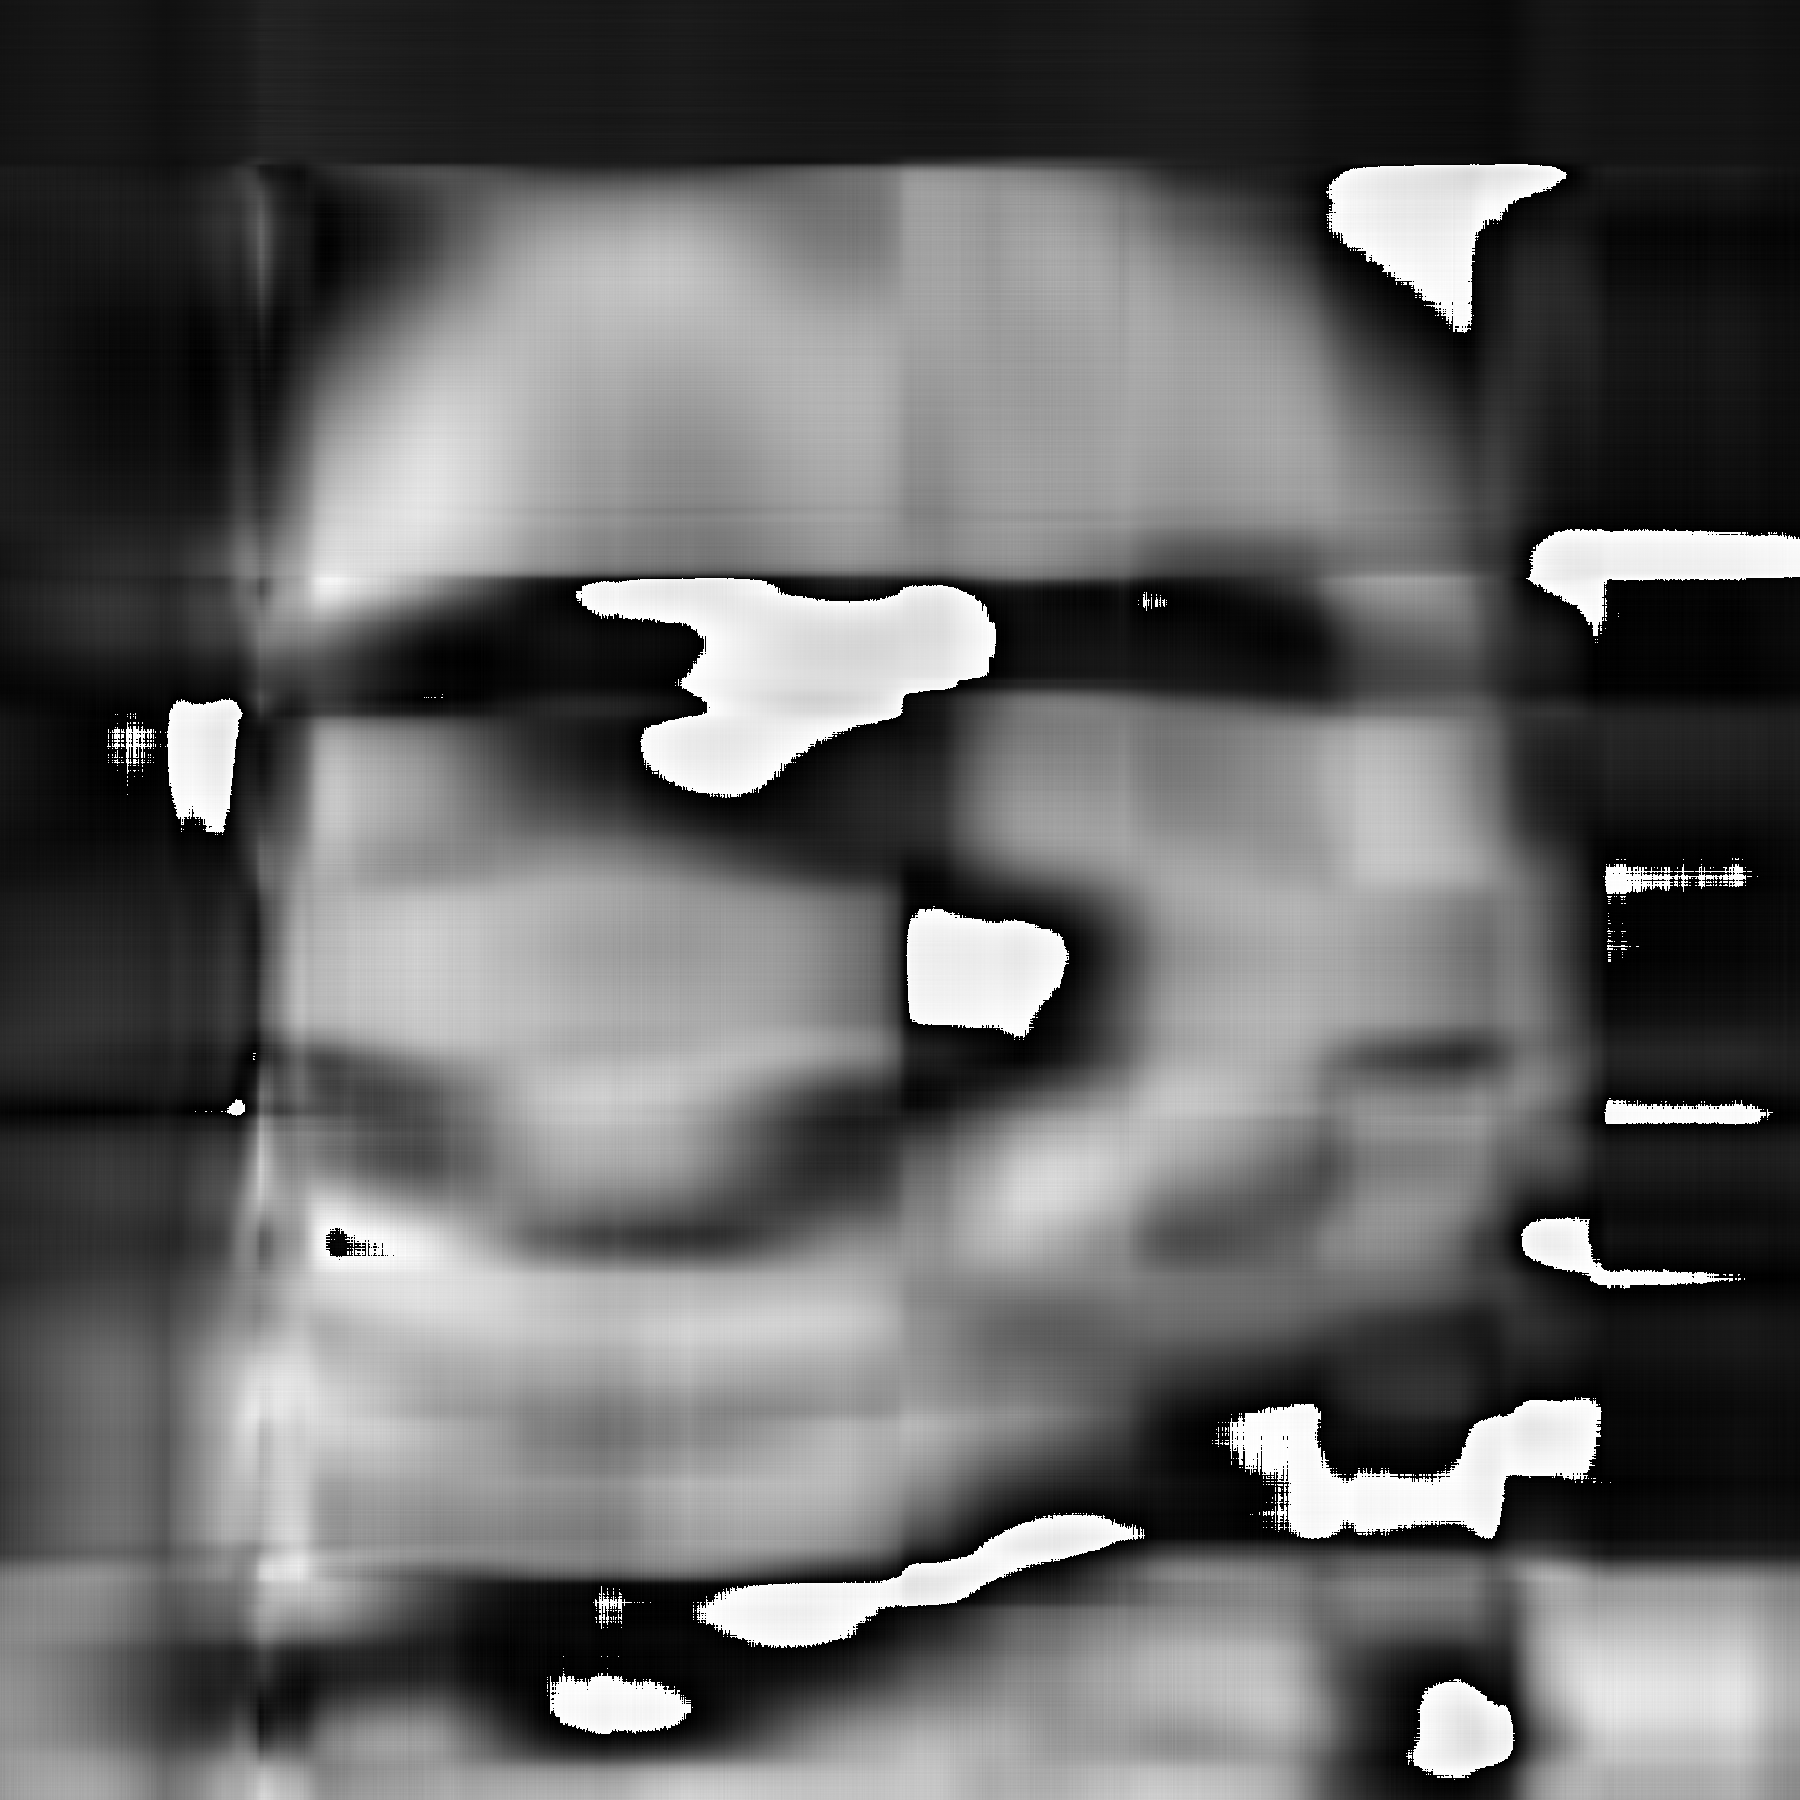
\includegraphics[width=0.3\textwidth]{approx06.png} &
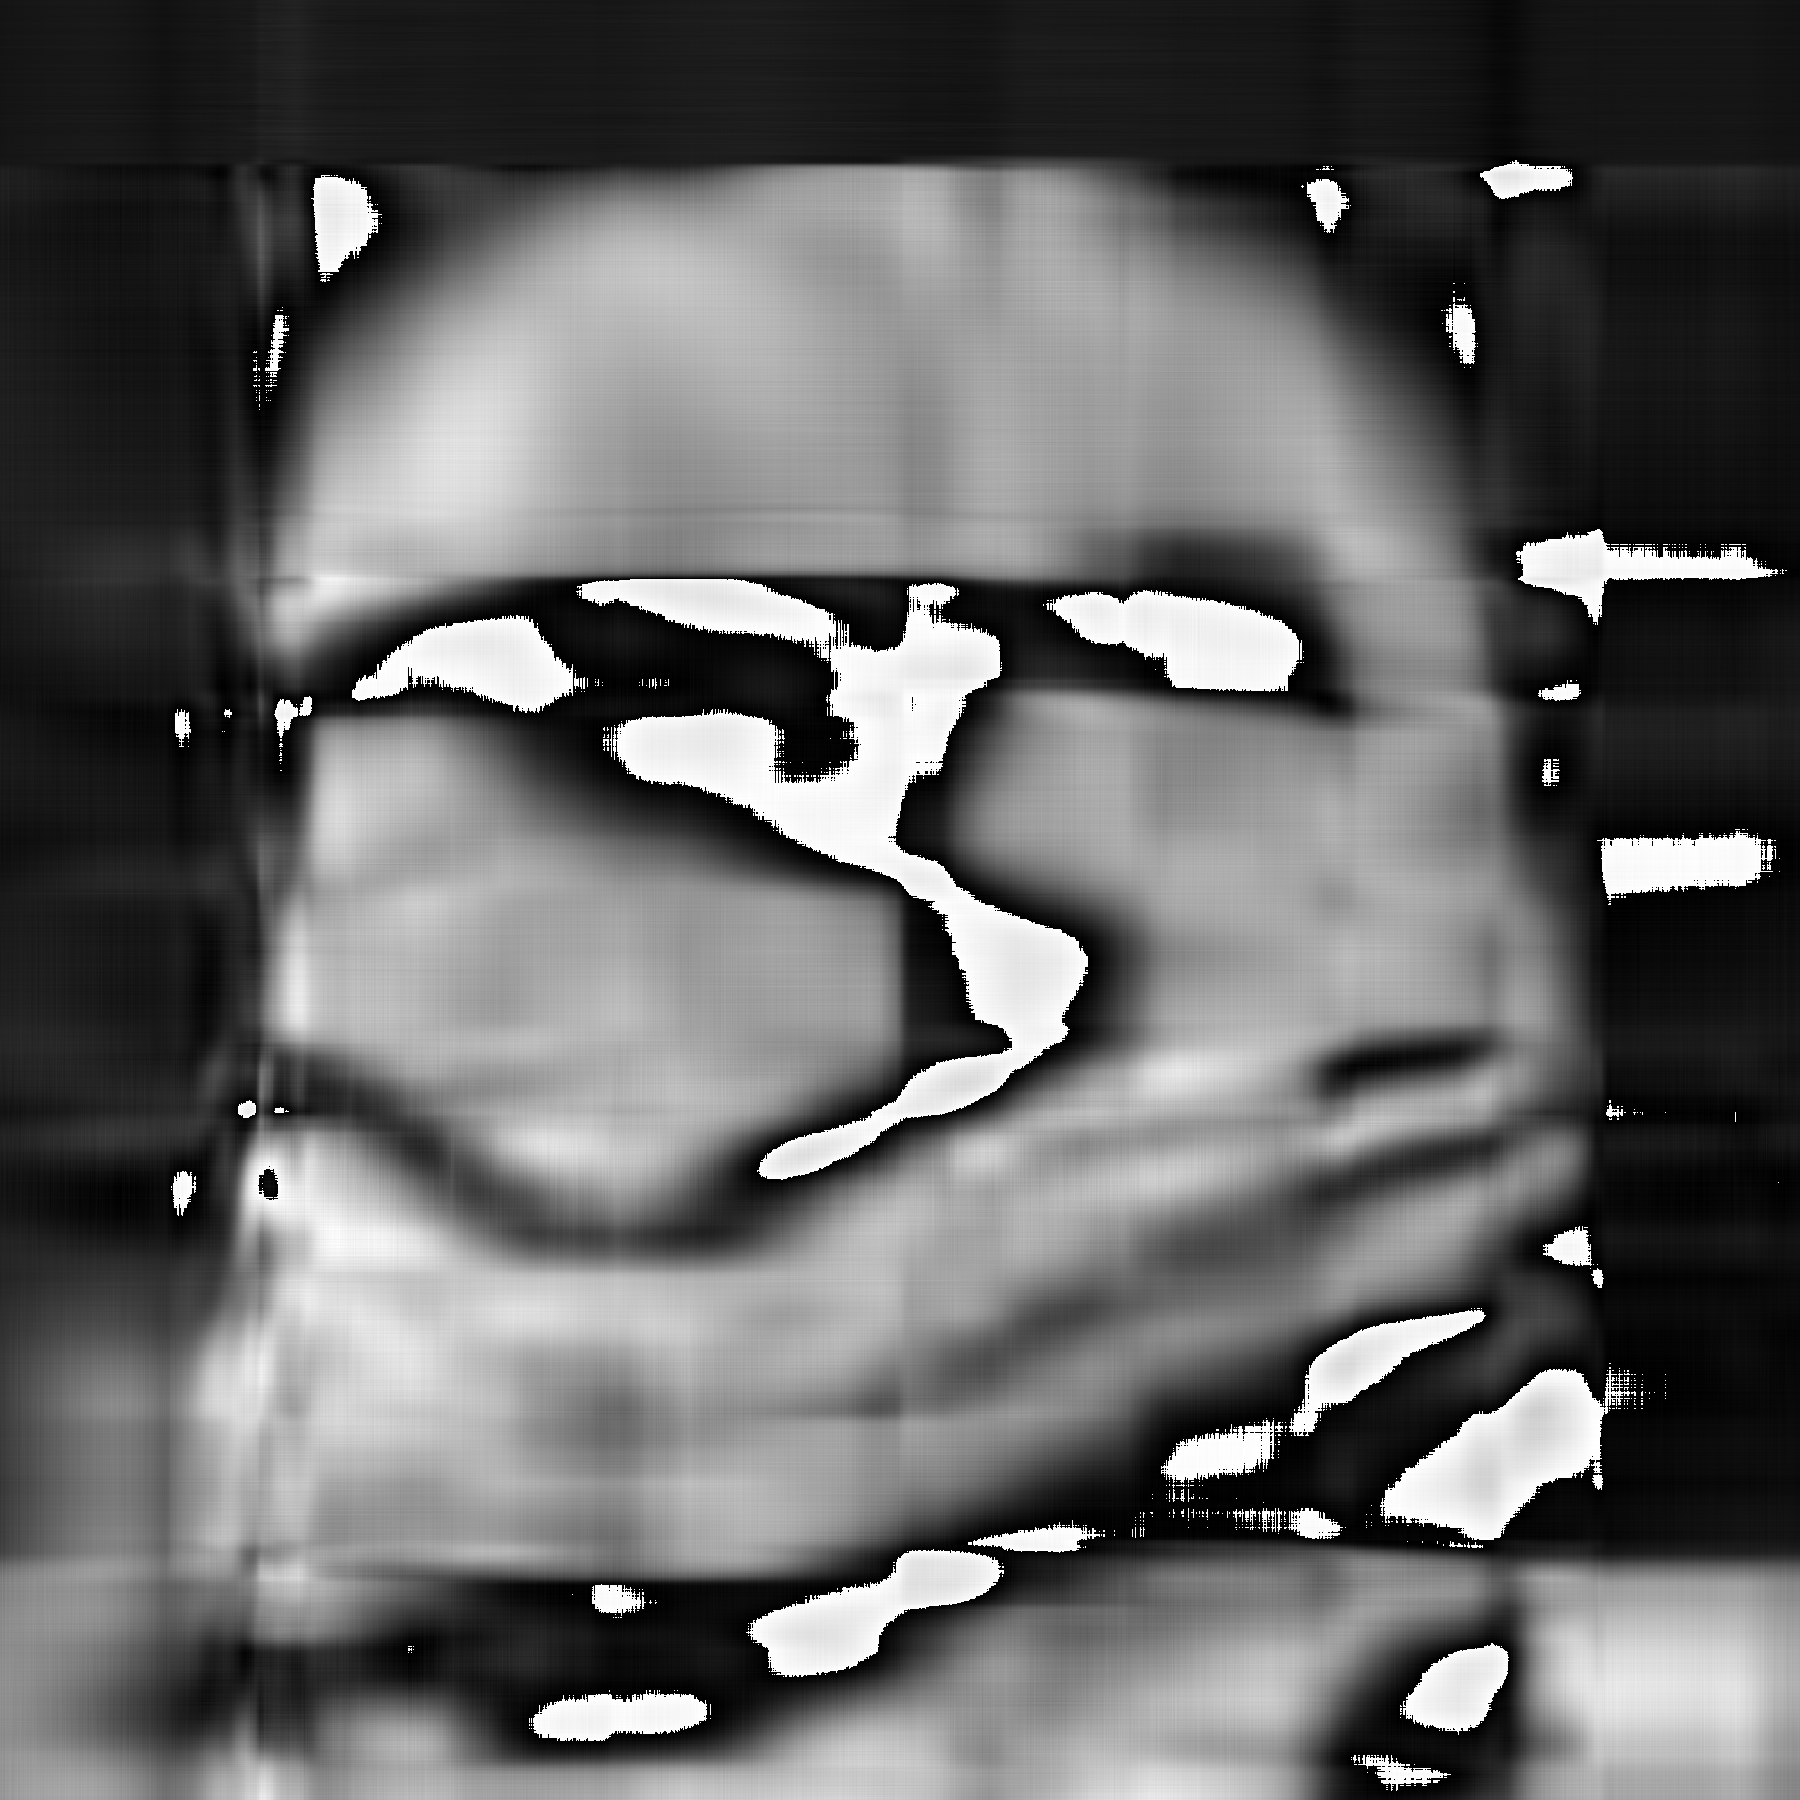
\includegraphics[width=0.3\textwidth]{approx09.png} &
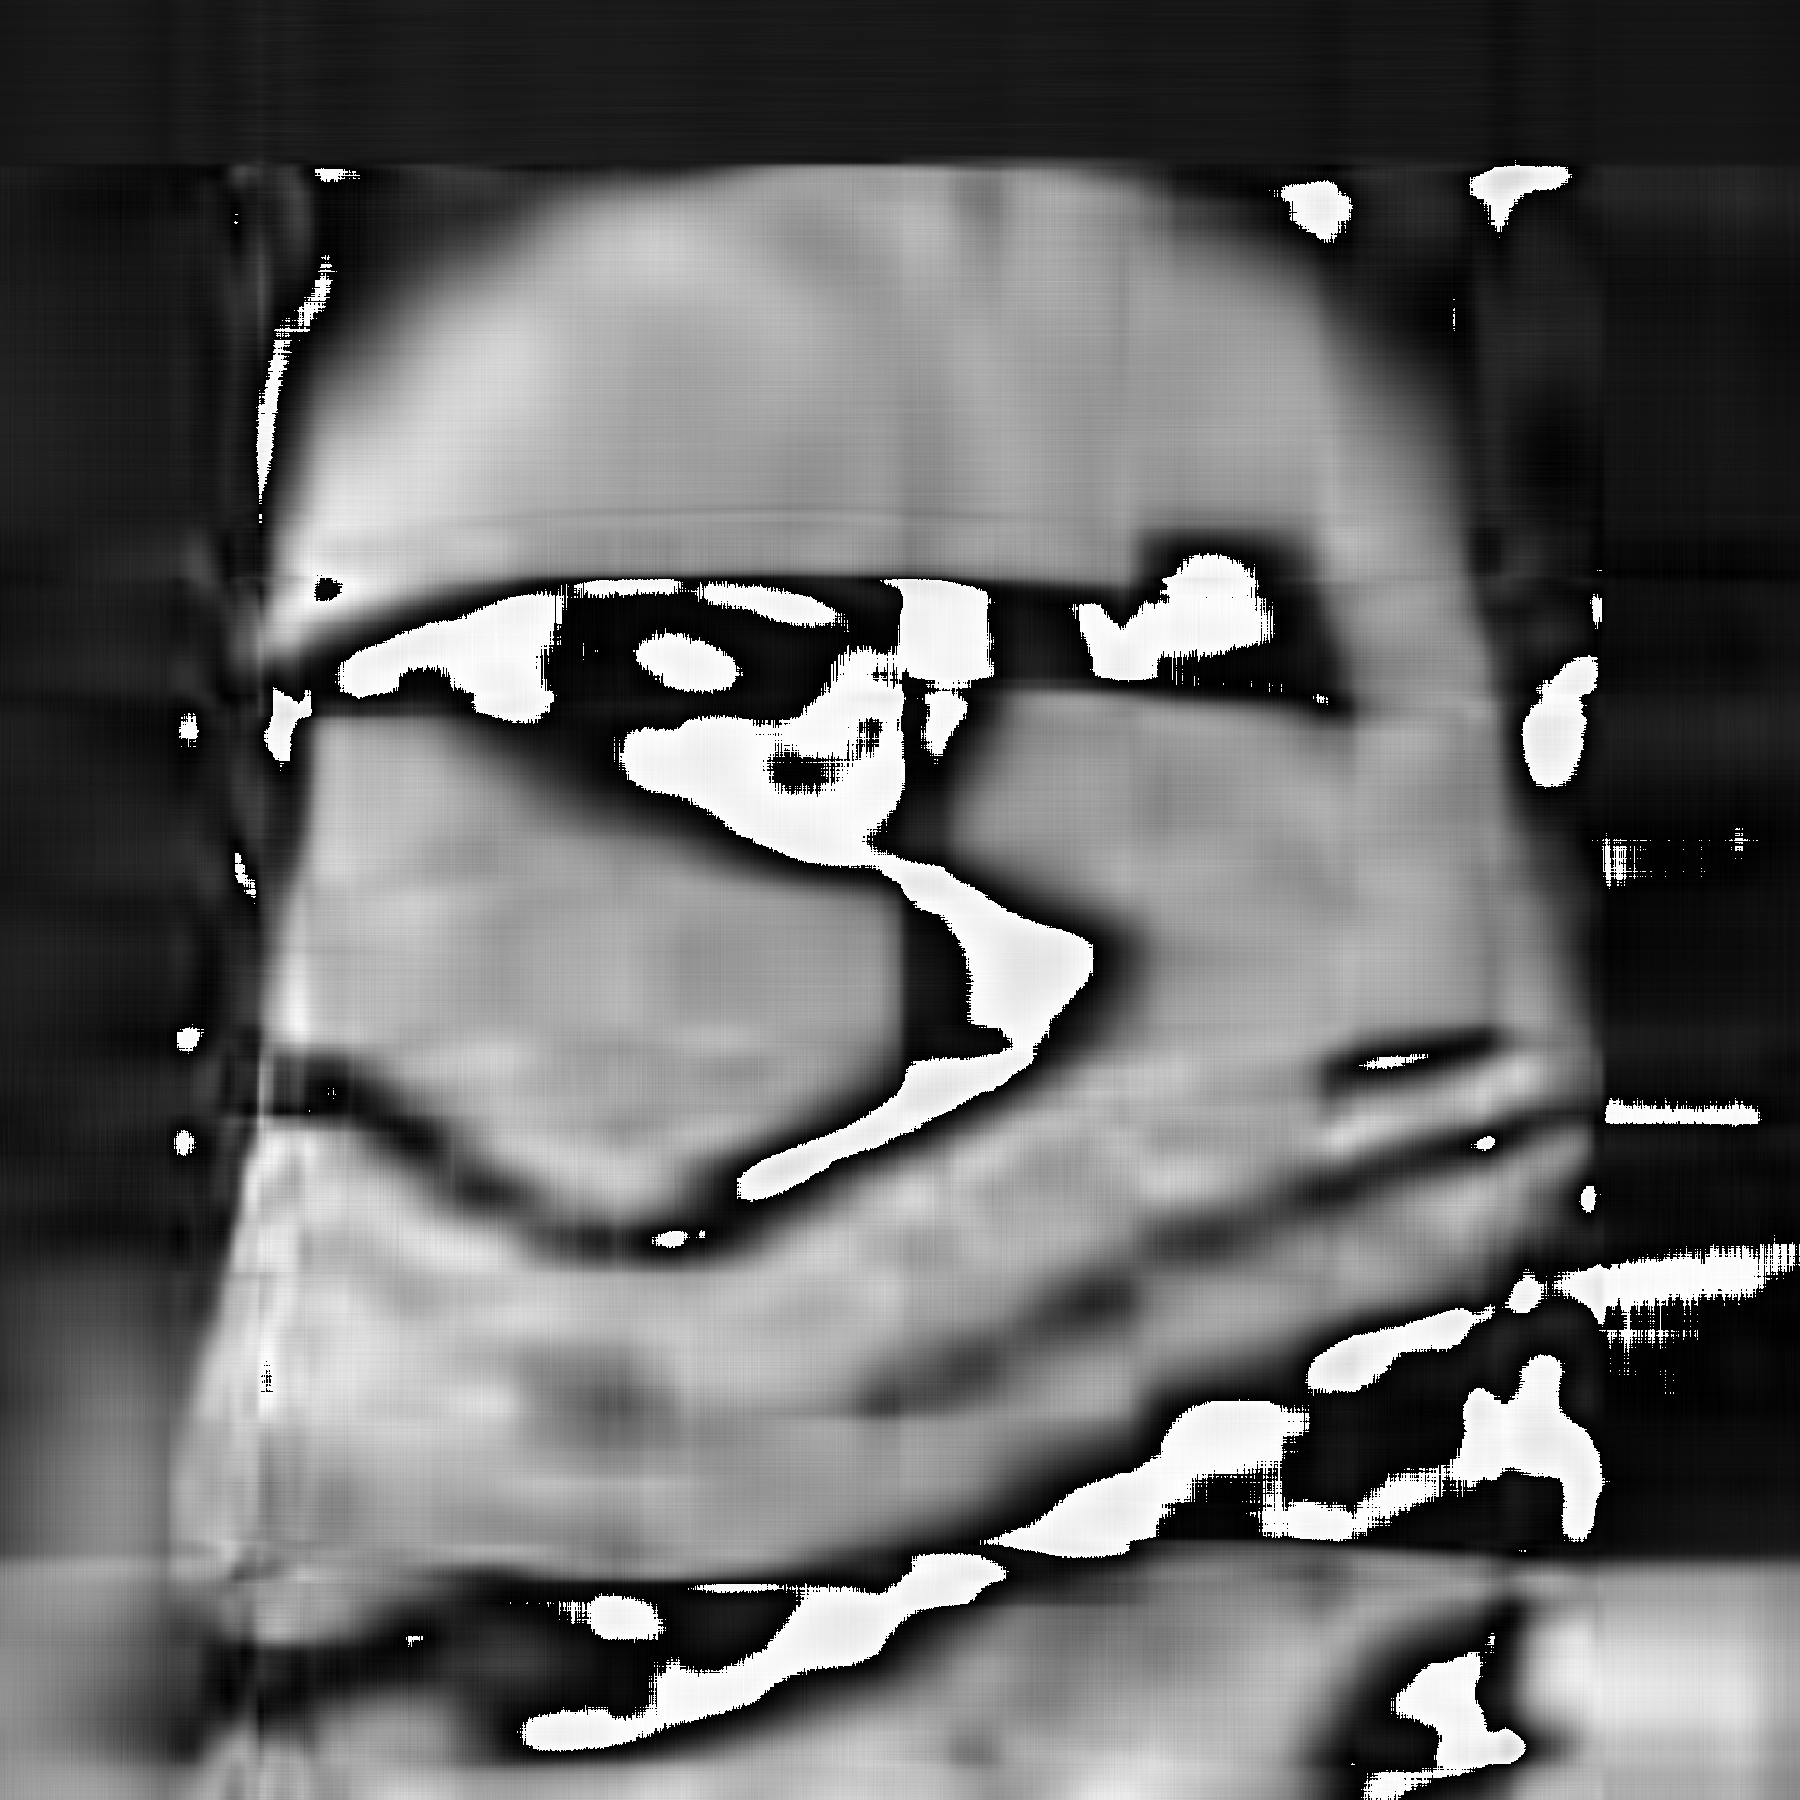
\includegraphics[width=0.3\textwidth]{approx12.png}\\
\smallskip
\scriptsize{Rank-20 (72,000 bytes)} &
\scriptsize{Rank-30 (108,000 bytes)} &
\scriptsize{Rank-40 (144,000 bytes)} \\

\includegraphics[width=0.3\textwidth]{approx20.png} &
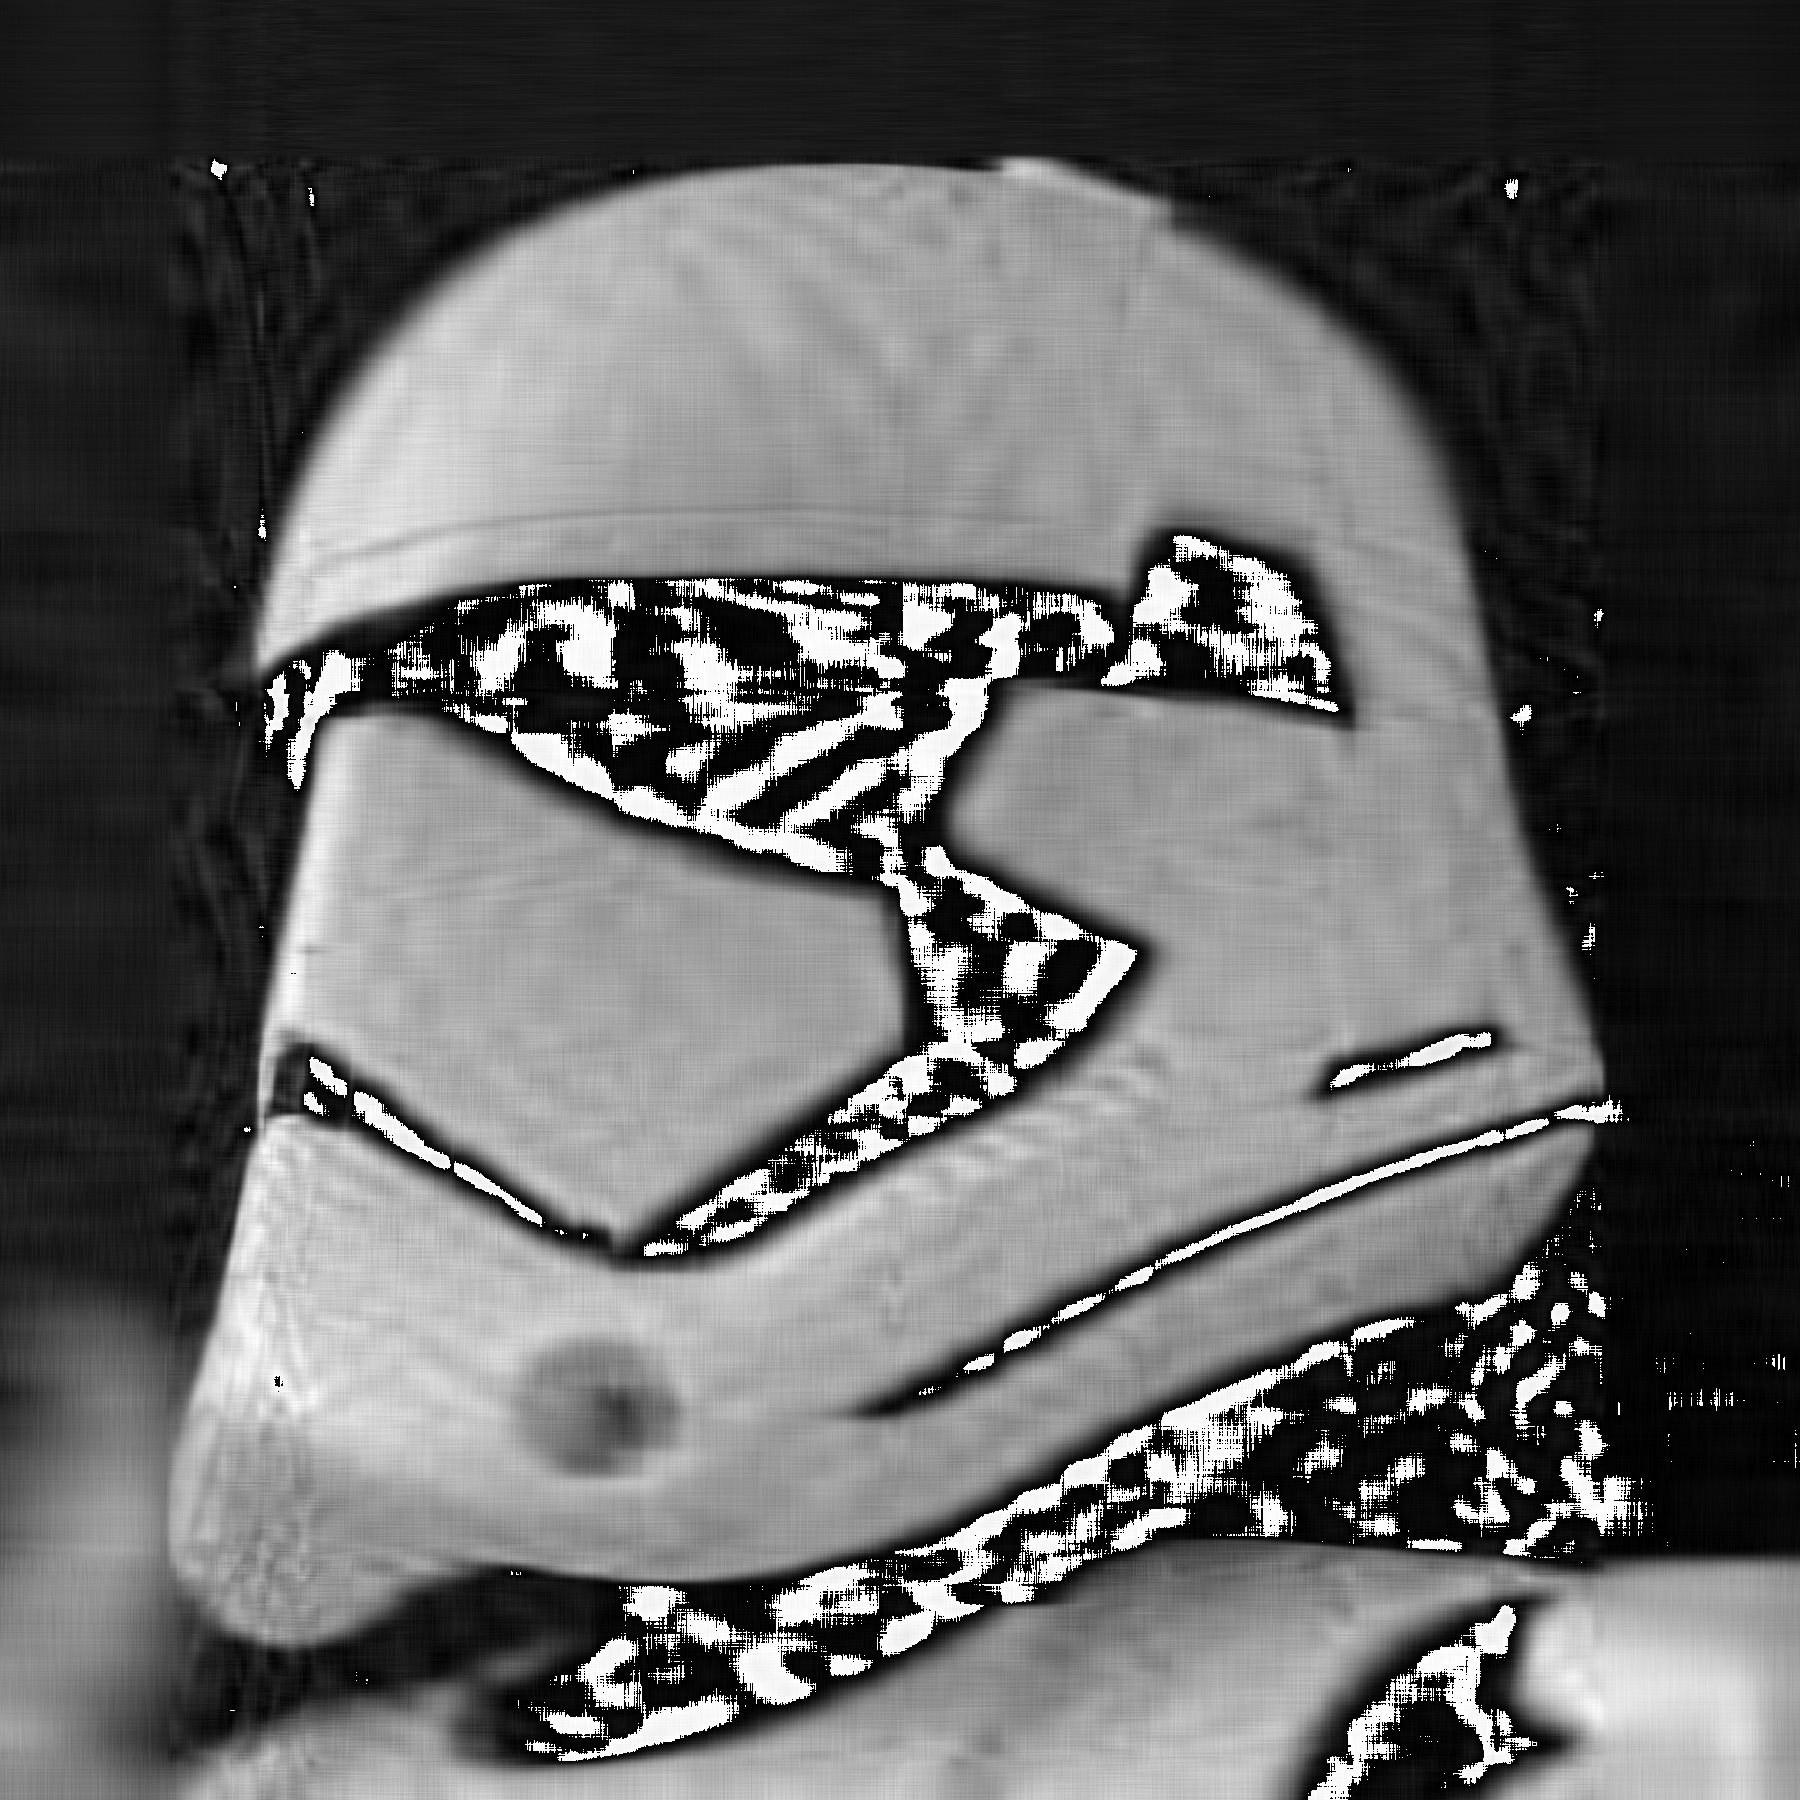
\includegraphics[width=0.3\textwidth]{approx30.png} &
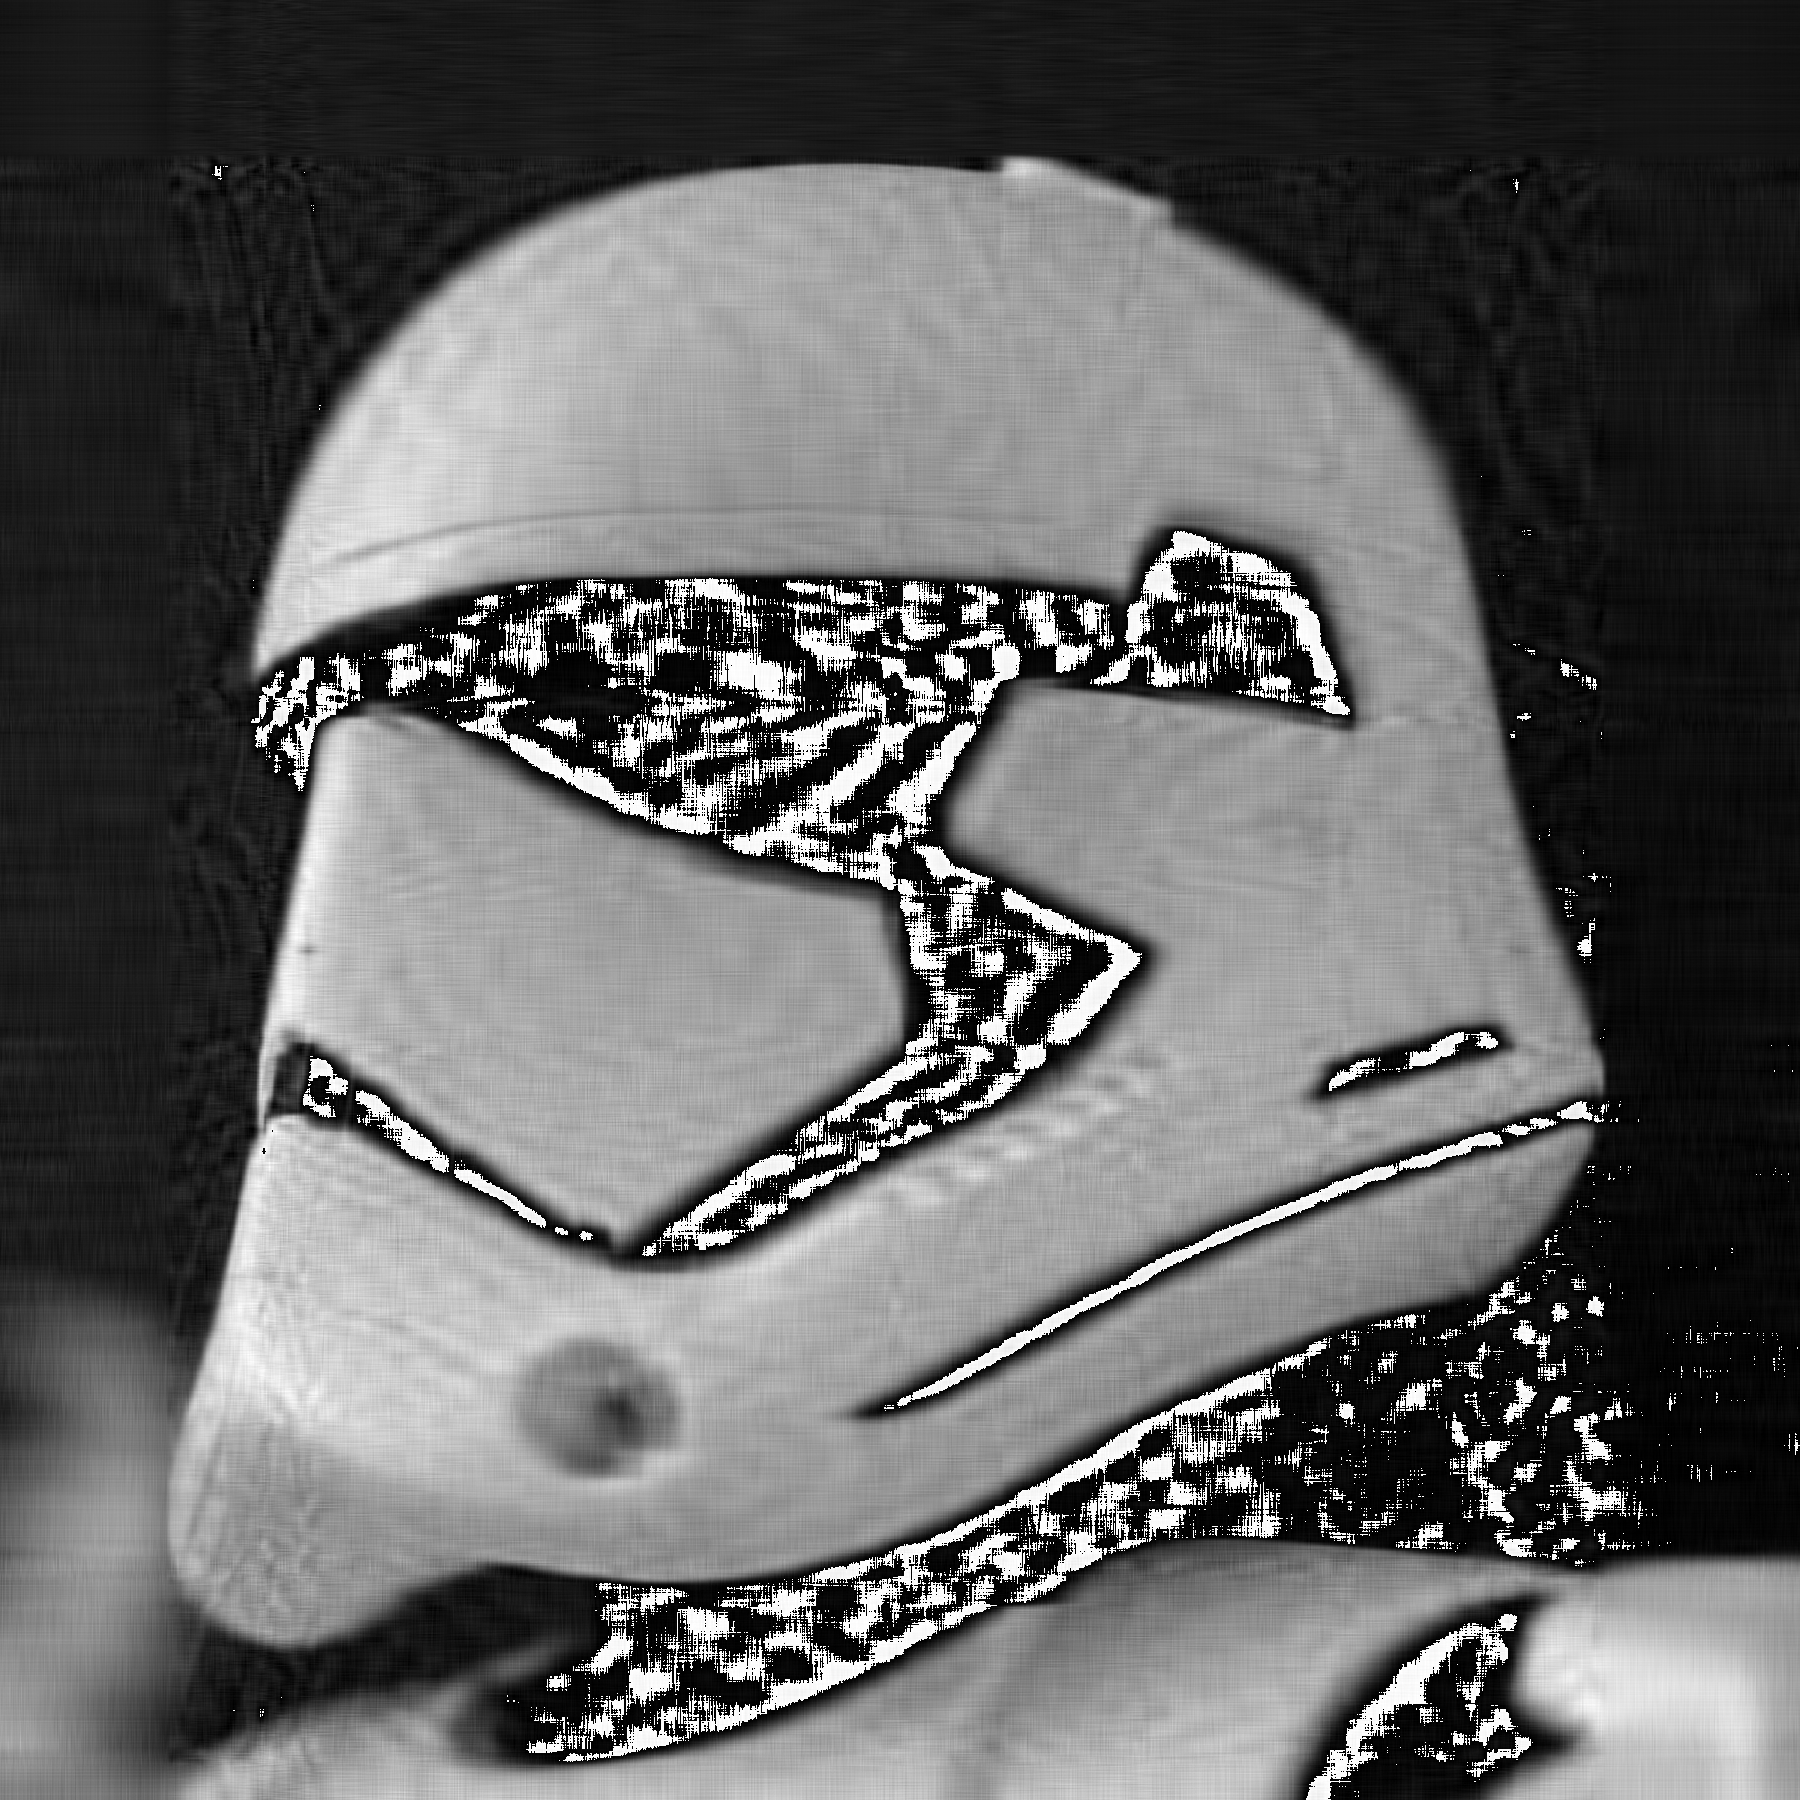
\includegraphics[width=0.3\textwidth]{approx40.png}\\
\scriptsize{Rank-100 (360,000 bytes)} &
\scriptsize{Rank-200 (720,000 bytes)} &
\scriptsize{Rank-400 (1,440,000 bytes)} \\
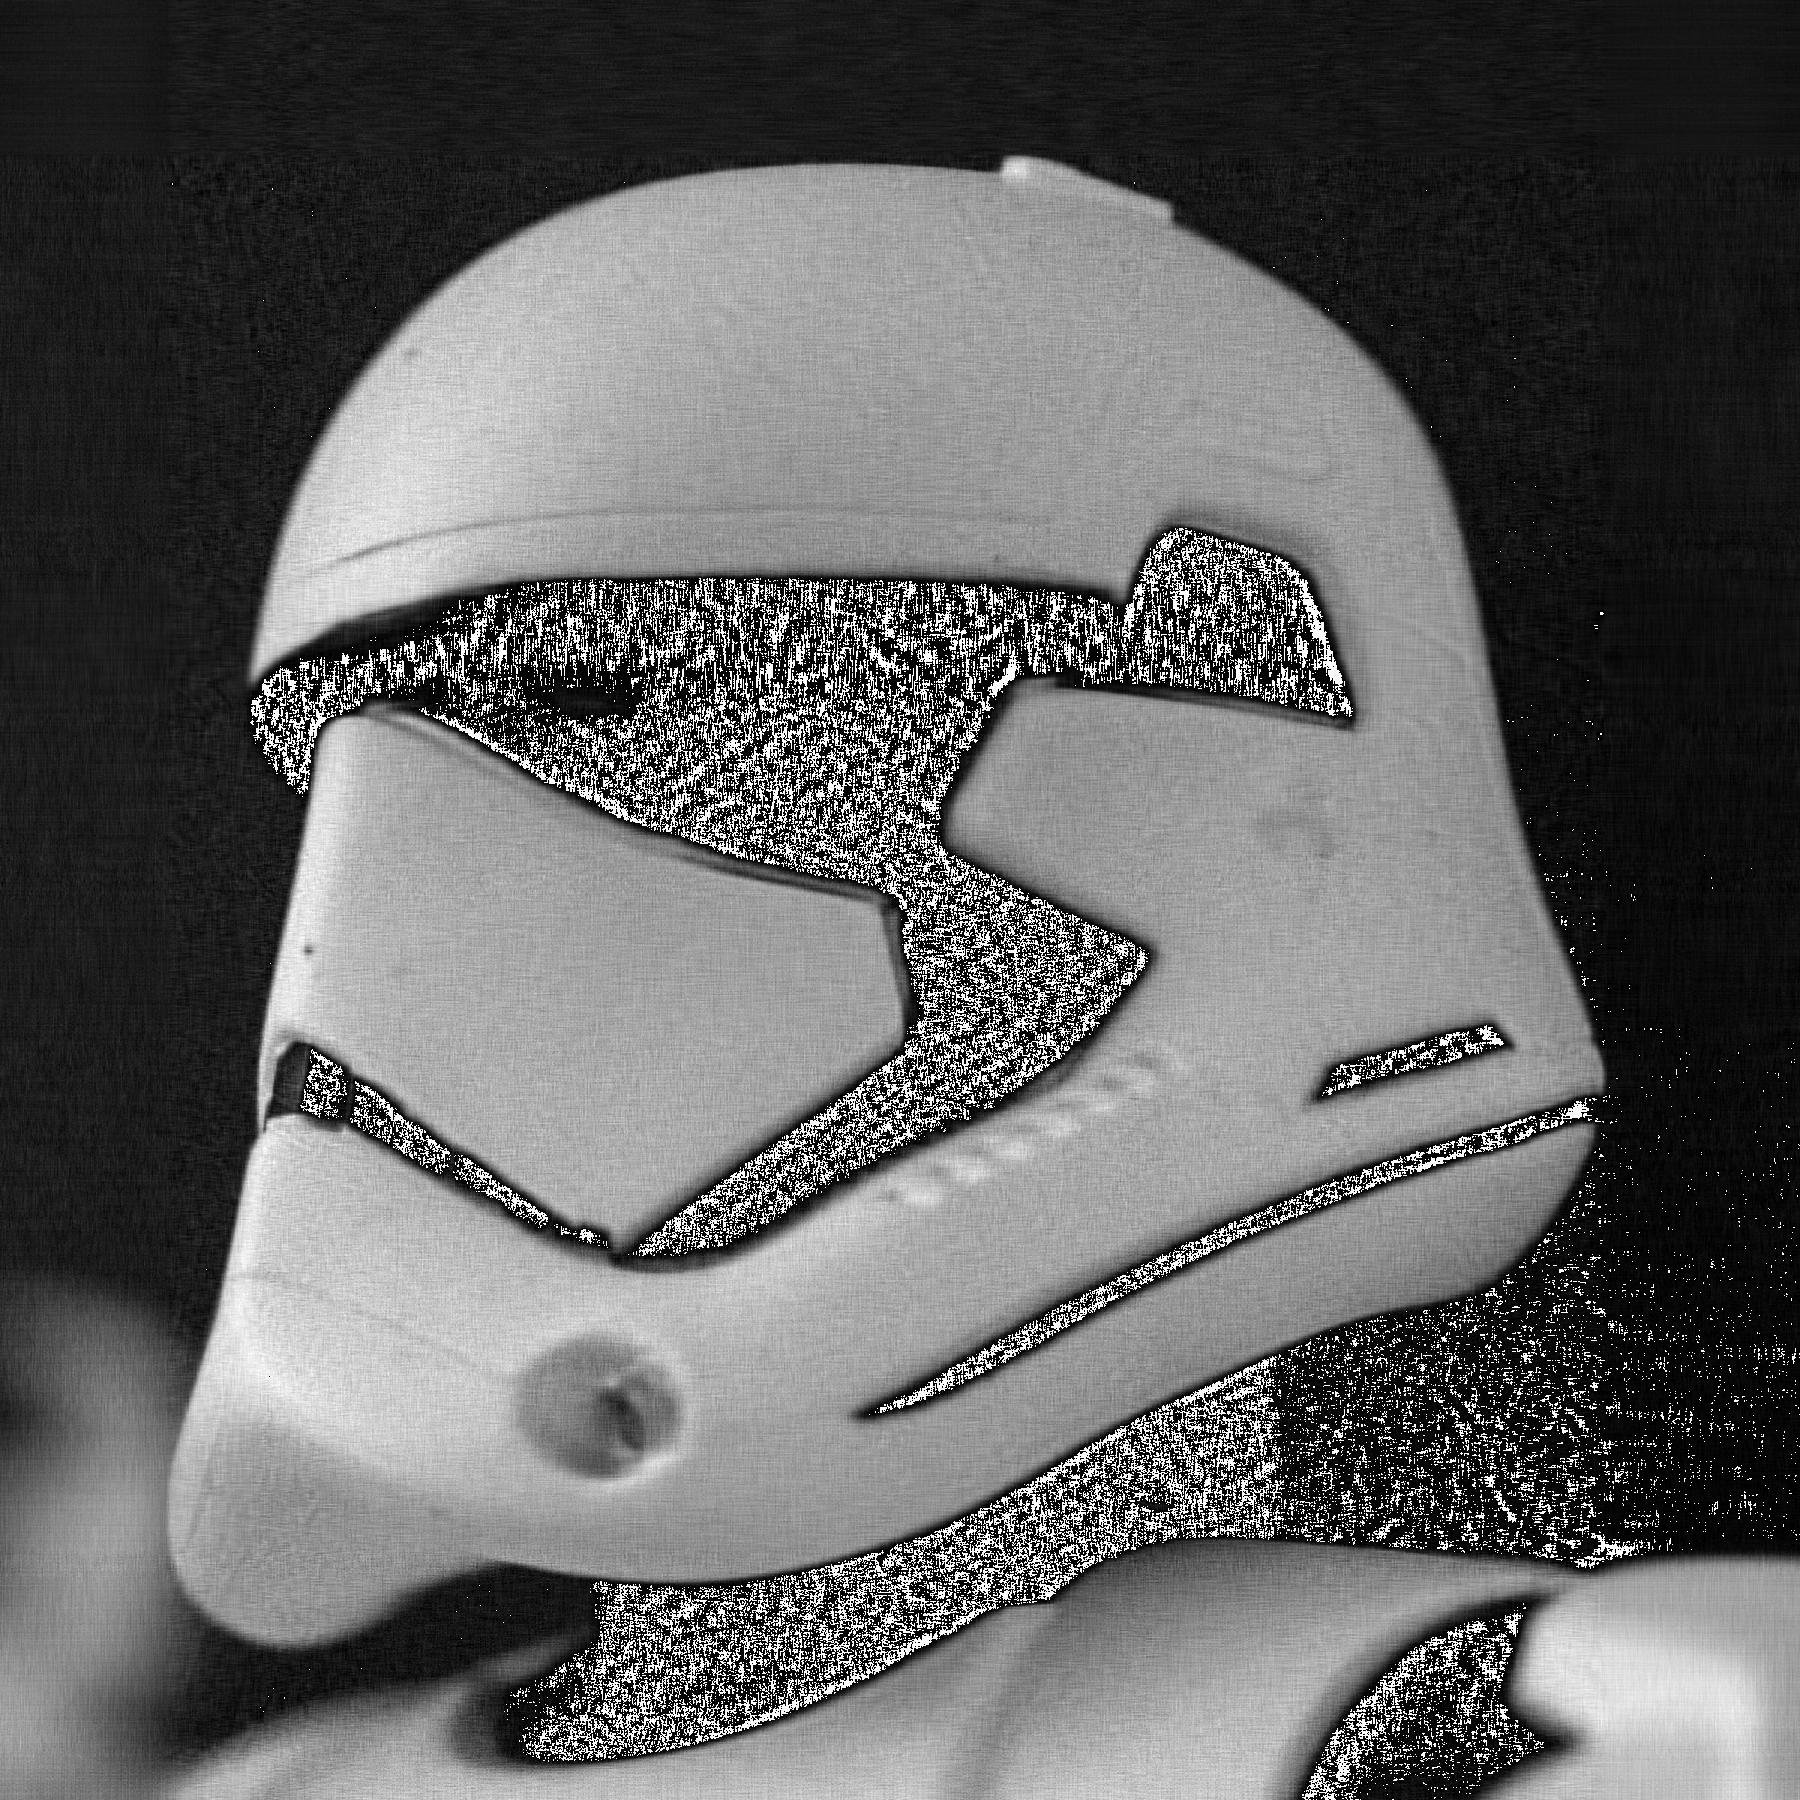
\includegraphics[width=0.3\textwidth]{approx100.png} &
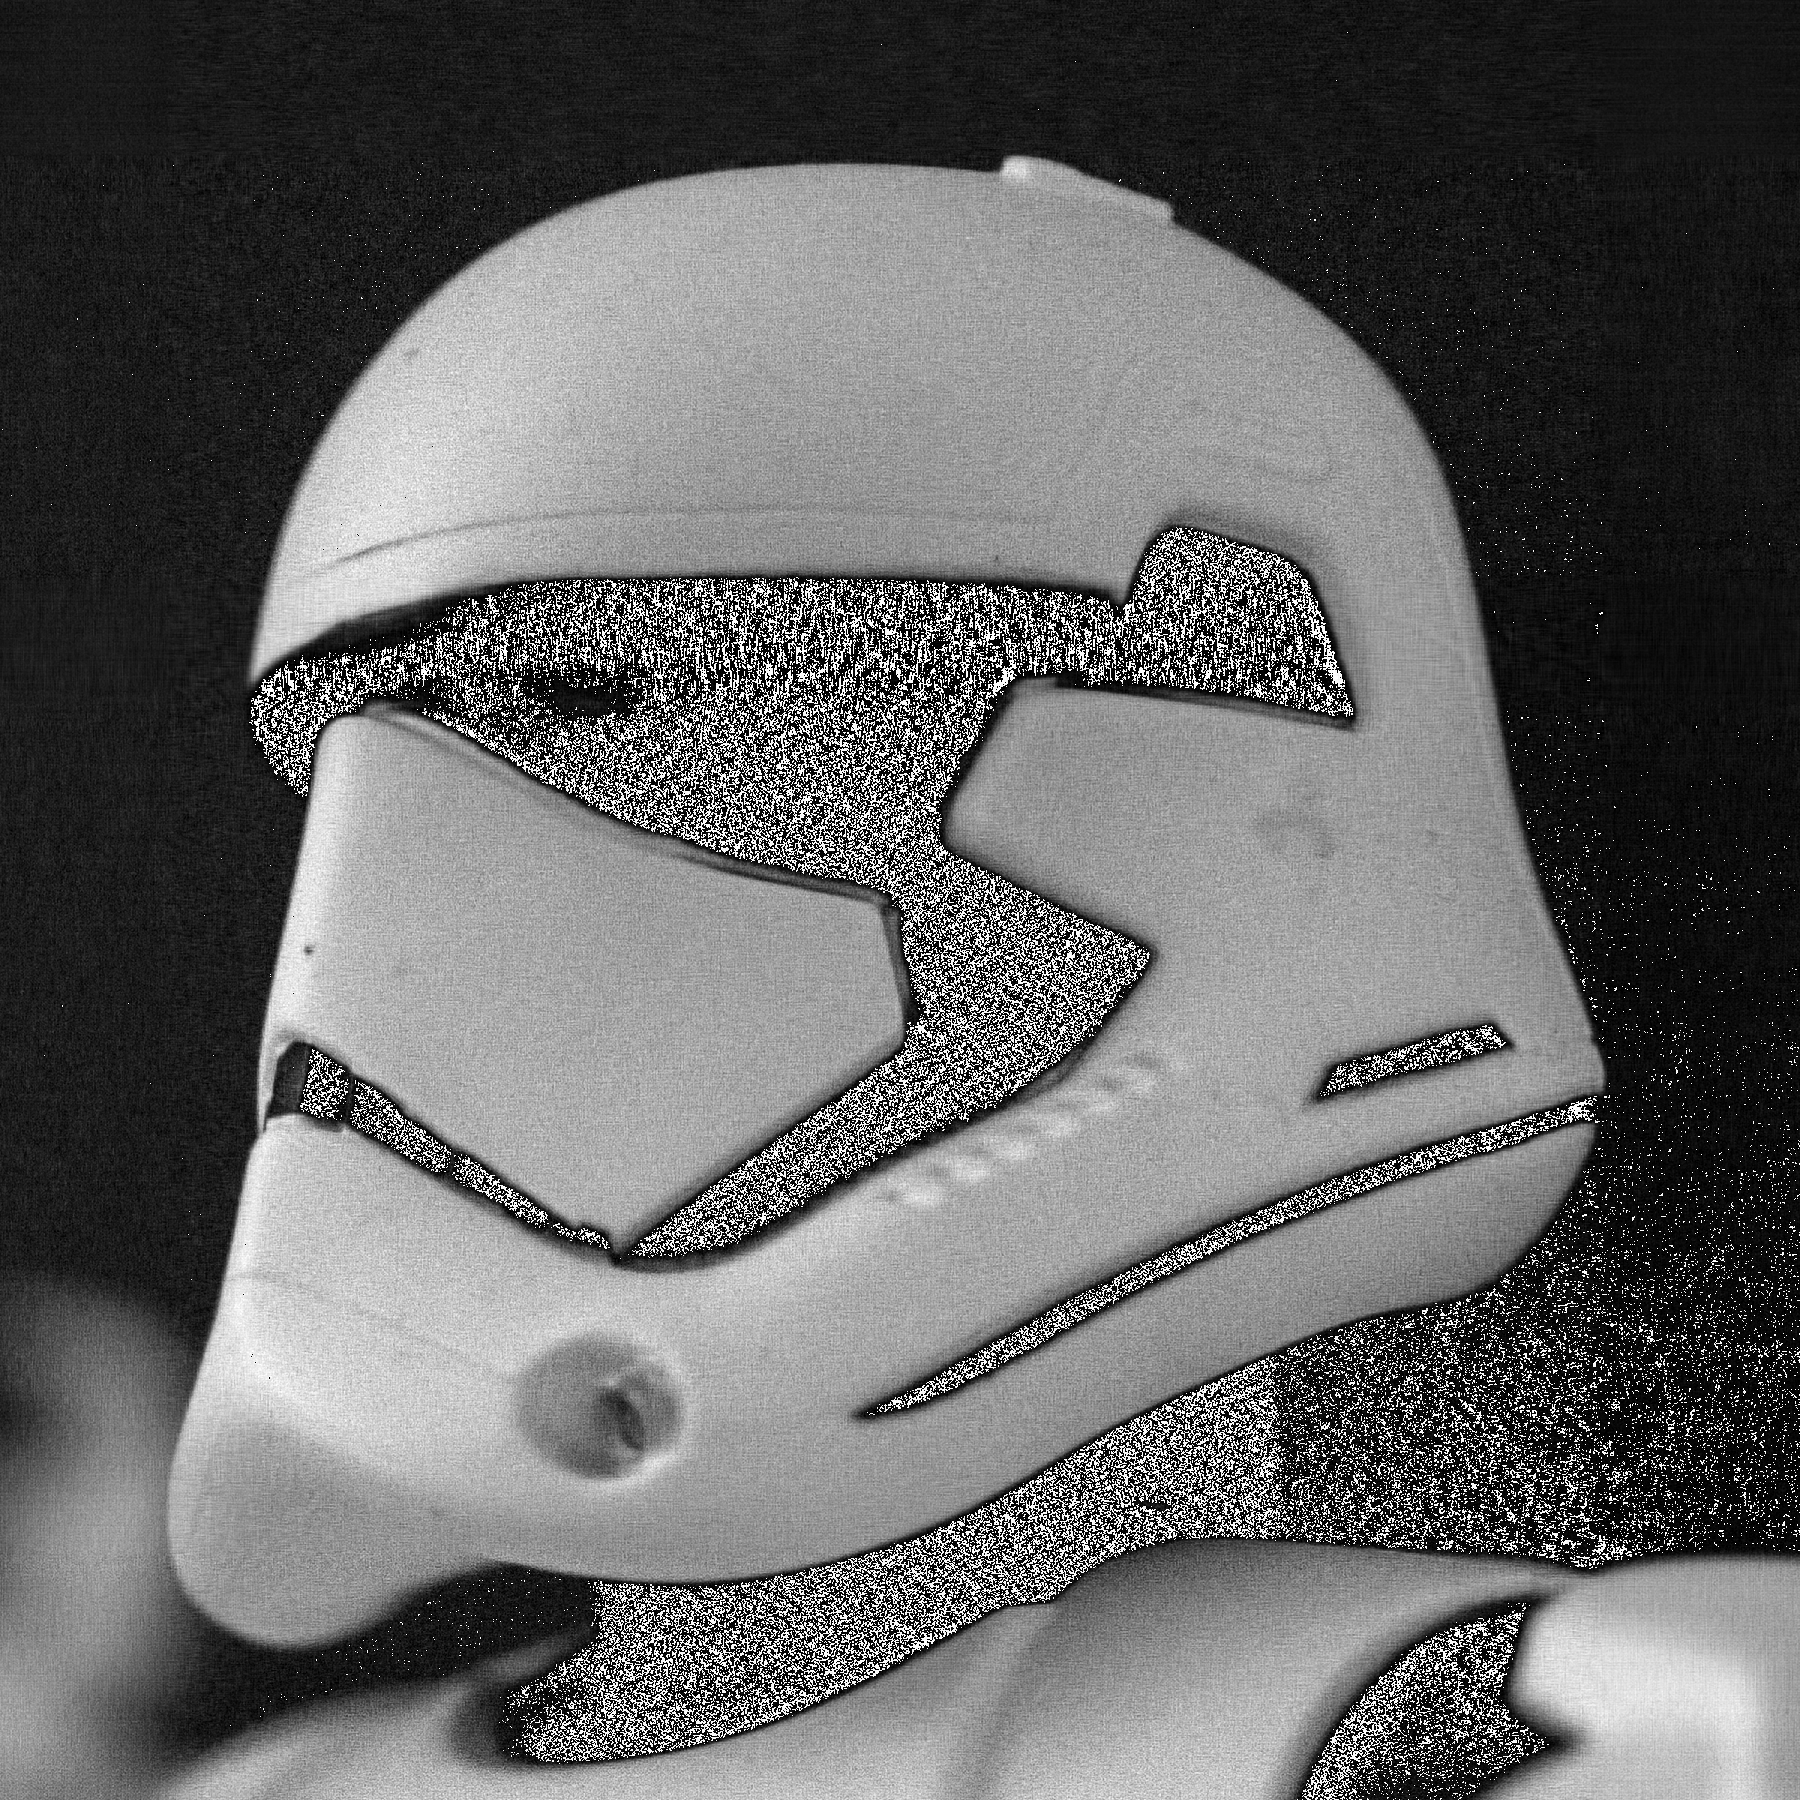
\includegraphics[width=0.3\textwidth]{approx200.png} &
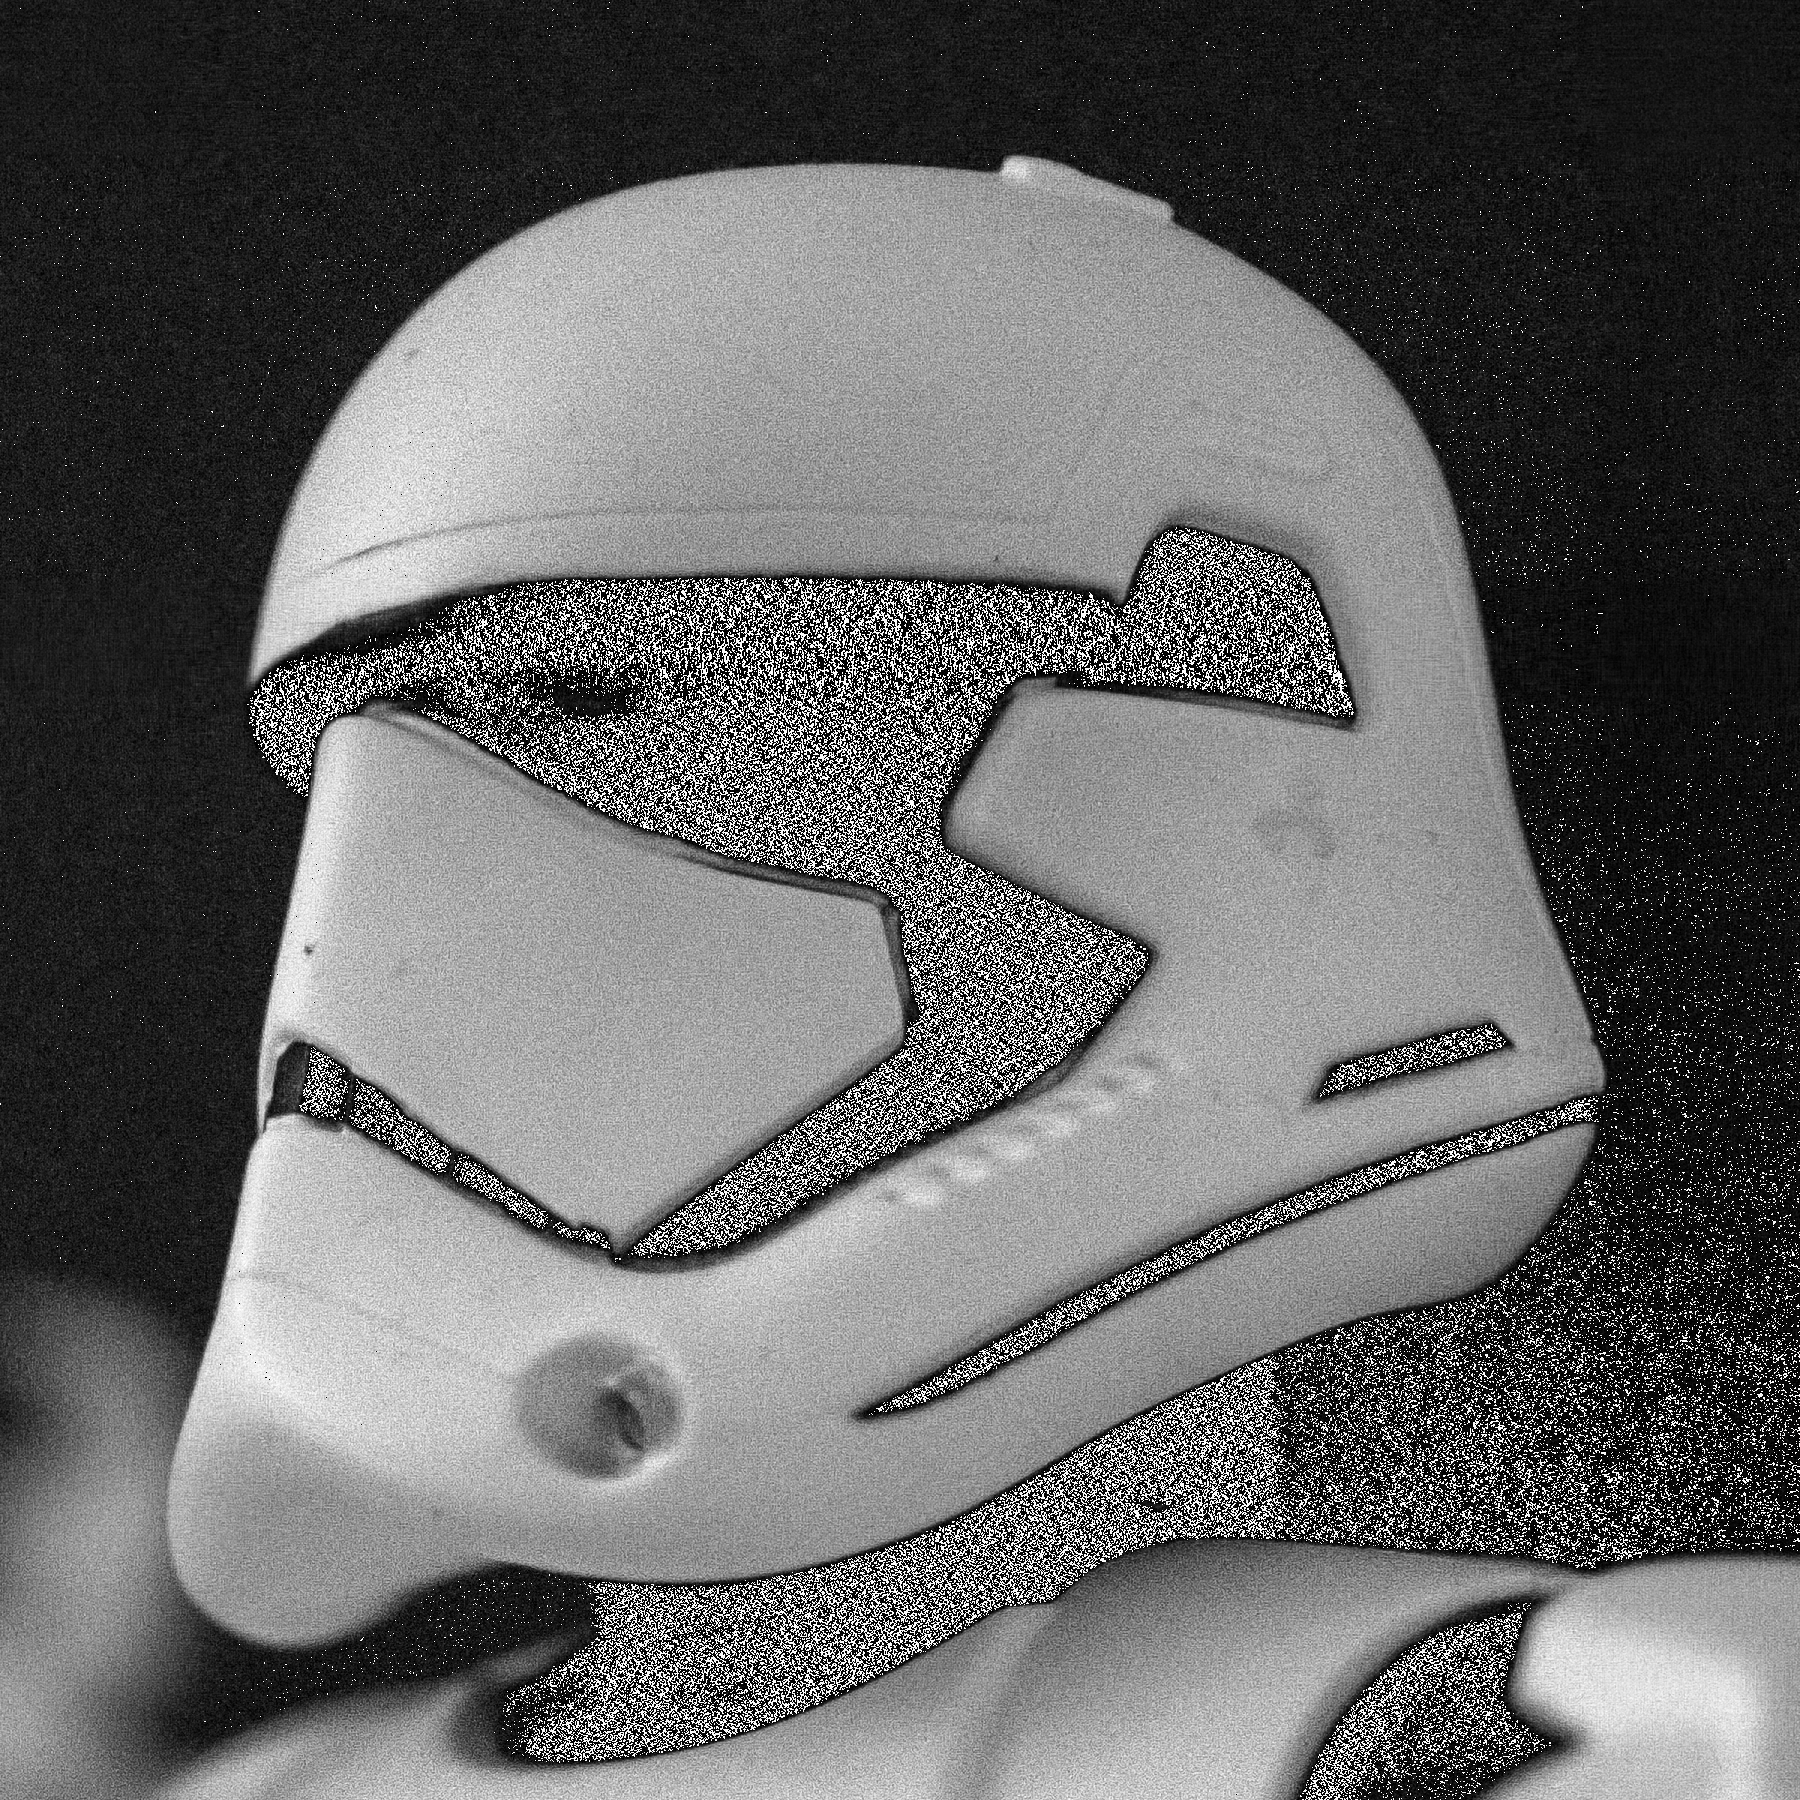
\includegraphics[width=0.3\textwidth]{approx400.png}\\
\end{tabular}
\caption{Low-rank approximations of an image matrix, using increasing numbers
of eigenvectors (and thus an increasing rank, with increasing
storage/transmission costs.)}
\label{fig:approximations}
\end{figure}

\pagebreak

It's interesting to watch how the image emerges as we add more eigenvectors.
With only the dominant eigenvector, all we can make out is a blurry,
right-angle-centric splash of black and white. Still, it's not bad for a rank-1
matrix, and after adding just a few more eigenvectors we can already see the
basic shape of the helmet come through.

Another observation is that we pretty quickly reach a point of diminishing
returns. Compare the rank-100 and rank-400 matrices in the bottom row of
Figure~\ref{fig:approximations}. Is it really worth quadrupling the size to get
the second one?

\begin{figure}[H]
\centering
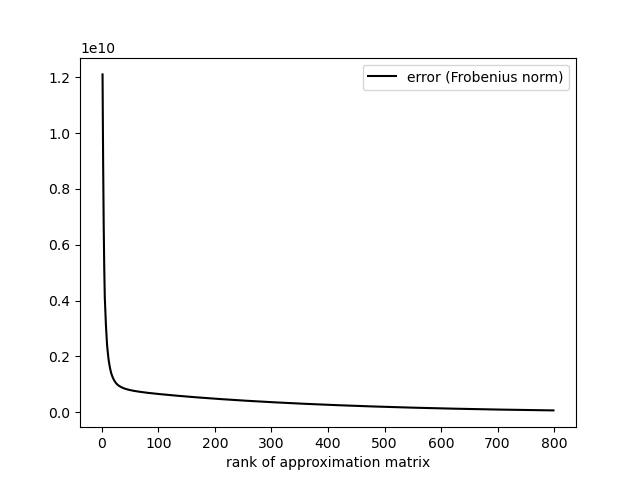
\includegraphics[width=0.7\textwidth]{frobenius.png}
\caption{The closeness to the original matrix as a function of the
approximation's rank.}
\label{fig:frobenius}
\end{figure}

Figure~\ref{fig:frobenius} quantifies this by plotting the rank of the matrix
against the Frobenius norm of the difference from the original. As you can see, 
less than fifty or so eigenvectors (out of the total of 1800) is enough to
eliminate nearly all the error.

% SVD/PCA
%   least squares approximation

% Markov chains

% PageRank

\end{alttitles}
